% 翻译成英文并保留latex命令:
% !Mode:: "TeX:UTF-8"
\chapter{Pre-integration}
\label{cpt:preinteg}
\thispagestyle{empty}
In Chapter~\ref{cpt:ins}~, we introduced the observation model of IMU data and basic filter methods. In ESKF, we integrate the IMU data between two GNSS observations as the prediction process of ESKF. This approach treats IMU data as a \textbf{one-time} usage: integrating them into the current estimate and then updating the estimate with observation data. Obviously, this method is related to the current state estimate. However, if the state variables change, can we reuse these IMU data? From a physical perspective, IMU reflects the \textbf{angular change} and \textbf{velocity change} of the vehicle between two moments. If we want the IMU computation to be independent of \textbf{the current state estimate}, how should we handle it algorithmically? This is the topic we will discuss in this chapter.

This chapter introduces a very common IMU data processing method: \textbf{Pre-integration} \cite{Forster2015}. Unlike traditional kinematic integration of IMU, pre-integration can accumulate IMU measurement data over a period of time to establish pre-integrated measurements while ensuring that the measurements are independent of state variables. To use an analogy, ESKF is like \textbf{eating dishes one bite at a time}, while pre-integration is \textbf{first picking pieces of food from the pot into a bowl and then eating all the food in the bowl in one go}. As for how big the bowl should be and how many times to pick food before eating it all at once, the form is relatively flexible. Whether in LIO or VIO systems, pre-integration has become a standard method in many tightly coupled IMU systems \cite{Chang2020,Yuan2019,Eckenhoff2019}, but its principle is more complex compared to the traditional ESKF prediction process. Below, we will derive its basic principles and then implement a pre-integration system to solve the same problem as in the previous chapter. The content of this chapter serves as preparatory knowledge for many subsequent chapters, so readers must master it thoroughly.

\includepdf[width=\textwidth]{art/ch4.pdf}

\section{Pre-integration of IMU States}
\subsection{Definition of Pre-integration}
We still start from the kinematic model of IMU. In an IMU system, we consider five variables: rotation $\bm{R}$, translation $\bm{p}$, angular velocity $\boldsymbol{\omega}$, linear velocity $\bm{v}$, and acceleration $\bm{a}$. According to the kinematics introduced in Section~\ref{sec:math-basics}, the kinematic relationships of these variables can be written as \cite{Murray2017}:
\begin{subequations}\label{key}
	\begin{align}
		\dot{\bm{R}} &= \bm{R} \boldsymbol{\omega}^\wedge, \\
		\dot{\bm{p}} &= \bm{v}, \\
		\dot{\bm{v}} &= \bm{a}.
	\end{align}
\end{subequations}

Within the time interval $t$ to $t+\Delta t$, applying Euler integration to the above equations yields:
\begin{subequations}\label{key}
	\begin{align}
		\bm{R}(t+\Delta t) &= \bm{R}(t) \mathrm{Exp} (\boldsymbol{\omega}(t) \Delta t), \\
		\bm{v}(t+\Delta t) &= \bm{v}(t) + \bm{a}(t) \Delta t, \\
		\bm{p}(t+\Delta t) &= \bm{p}(t) + \bm{v}(t) \Delta t + \frac{1}{2} \bm{a}(t) \Delta t^2.
	\end{align}
\end{subequations}

Here, the angular velocity and acceleration can be measured by the IMU but are affected by noise and gravity. Let the measurements be $\tilde{\boldsymbol{\omega}}$ and $\tilde{\bm{a}}$, then:
\begin{subequations}\label{key}
	\begin{align}
		\tilde{\boldsymbol{\omega}}(t) &= \boldsymbol{\omega}(t) + \bm{b}_g (t) + \boldsymbol{\eta}_g 
		(t), \\
		\tilde{\bm{a}}(t) &= \bm{R}^\top (\bm{a}(t) - \bm{g}) + \bm{b}_a (t) + \boldsymbol{\eta}_a 
		(t),
	\end{align}
\end{subequations}
where $\bm{b}_g, \bm{b}_a$ are the biases of the gyroscope and accelerometer, and $\boldsymbol{\eta}_a, \boldsymbol{\eta}_g$ are Gaussian measurement noises. Substituting these into the above equations, we obtain the relationship between the measurements and the state variables:
\begin{subequations}\label{eq:kinematics-delta-t}
	\begin{align}
		\bm{R}(t+\Delta t) &= \bm{R}(t) \mathrm{Exp} \left((\tilde{\boldsymbol{\omega}} - \bm{b}_g(t) - 
		\boldsymbol{\eta}_{gd} (t))\Delta t \right), \\
		\bm{v}(t+\Delta t) &= \bm{v}(t) + \bm{g} \Delta t + \bm{R}(t) (\tilde{\bm{a}} -\bm{b}_a(t) - 
		\boldsymbol{\eta}_{ad}(t)) \Delta t, \\
		\bm{p}(t+\Delta t) &= \bm{p}(t) + \bm{v}(t) \Delta t + \frac{1}{2}\bm{g} \Delta t^2 + \frac{1}{2} 
		\bm{R}(t) (\tilde{\bm{a}} -\bm{b}_a(t) - \boldsymbol{\eta}_{ad}(t)) \Delta t^2 ,
	\end{align}
\end{subequations}
where $\boldsymbol{\eta}_{gd}, 
\boldsymbol{\eta}_{ad}$ are the discretized random walk noises \cite{Crassidis2006}:
\begin{subequations}\label{key}
	\begin{align}
		\mathrm{Cov}(\boldsymbol{\eta}_{gd}(t) ) &= \frac{1}{\Delta t} \mathrm{Cov} 
		(\boldsymbol{\eta}_g(t)), \\
		\mathrm{Cov}(\boldsymbol{\eta}_{ad}(t) ) &= \frac{1}{\Delta t} \mathrm{Cov} 
		(\boldsymbol{\eta}_a(t)).
	\end{align}
\end{subequations}

The above process has already been described in the IMU measurement and noise equations. Of course, we could directly use these constraints to construct graph optimization and solve IMU-related problems. However, these equations describe an extremely short time interval, involving only a single IMU measurement. In other words, the IMU measurement frequency is too high. We do not want the optimization process to be invoked with every IMU measurement, as that would waste computational resources. Instead, we prefer to process these IMU measurements collectively.

\section{Pre-integration of IMU States}
\subsection{Definition of Pre-integration}
Now we introduce how to perform IMU pre-integration between keyframes. Let us assume that IMU data between discrete times $i$ and $j$ are accumulated, a process that can last several seconds. This accumulated observation is called \textbf{pre-integration} \cite{Lupton2011}. Of course, if we use different forms of kinematics (such as those introduced in Section~\ref{sec:math-basics}), the resulting pre-integration forms will also differ \cite{Qin2018}. This book primarily uses the $\mathrm{SO}(3)+\bm{t}$ approach to derive pre-integration. Thus, during the interval from $i$ to $j$, we can accumulate the variables in Equation \eqref{eq:kinematics-delta-t} to obtain:
\begin{subequations}
	\begin{align}
		\bm{R}_j &= \bm{R}_i \prod_{k=i}^{j-1} \left(\mathrm{Exp} \left(\left( \tilde{\boldsymbol{\omega}}_k - 
		\bm{b}_{g,k} - \boldsymbol{\eta}_{gd, k} \right) \Delta t \right)\right), \\
		\bm{v}_j &= \bm{v}_i + \bm{g} \Delta t_{ij} + \sum_{k=i}^{j-1} \bm{R}_k (\tilde{\bm{a}}_k - 
		\bm{b}_{a, k} - \boldsymbol{\eta}_{ad, k}) \Delta t, \\
		\bm{p}_j &= \bm{p}_i + \sum_{k=i}^{j-1} \bm{v}_k \Delta t + \frac{1}{2} \sum_{k=i}^{j-1} \bm{g} \Delta t^2 + 
		\frac{1}{2} \sum_{k=i}^{j-1} \bm{R}_k (\tilde{\bm{a}}_k - \bm{b}_{a,k} - \boldsymbol{\eta}_{ad, k}) 
		\Delta t^2,
	\end{align}
\end{subequations}
where $\Delta t_{ij} = \sum_{k=i}^{j-1} \Delta t$ is the accumulated time. Given the state at time $i$ and all measurements, this equation can be used to infer the state at time $j$. Of course, this is merely the accumulated form of Equation \eqref{eq:kinematics-delta-t}, with no fundamental difference. This is the traditional \textbf{direct integration}, identical to the prediction process in ESKF.

The drawback of direct integration is that it describes a process dependent on the state variables. If we optimize the state at time $i$, the states at times $i+1, i+2, \ldots, j-1$ will also change, requiring this integration to be recalculated \cite{Leutenegger2015}, which is highly inconvenient. To address this, we slightly modify the above equations, striving to place IMU readings on one side and state variables on the other. Thus, we define relative motion quantities as follows:

\begin{subequations}
	\label{eq:def-preintegration}
	\begin{align}
		\Delta \bm{R}_{ij} & \buildrel\textstyle.\over= \bm{R}_i^\top \bm{R}_j = \prod_{k=i}^{j-1} 
		\mathrm{Exp} \left( \left(\tilde{\boldsymbol{\omega}}_k - \bm{b}_{g,k} - \boldsymbol{\eta}_{gd, 
			k}\right) \Delta t\right), \\
		\Delta \bm{v}_{ij} &\buildrel\textstyle.\over= \bm{R}_i^\top(\bm{v}_j - \bm{v}_i -\bm{g} 
		\Delta t_{ij}) = \sum_{k=i}^{j-1} \Delta \bm{R}_{ik} (\tilde{\bm{a}}_k - \bm{b}_{a,k} - 
		\boldsymbol{\eta}_{ad, k}) \Delta t,\\
		\Delta \bm{p}_{ij} &\buildrel\textstyle.\over= \bm{R}_i^\top \left( \bm{p}_j - \bm{p}_i - 
		\bm{v}_i \Delta t_{ij} - \bm{g} \Delta t_{ij}^2 \right), \\
		&= \sum_{k=i}^{j-1} \left[\Delta \bm{v}_{ik} \Delta t+\frac{1}{2} \Delta \bm{R}_{ik} 
		\left(\tilde{\bm{a}}_k - \bm{b}_{a,k} - \boldsymbol{\eta}_{ad, k} \right)\Delta t^2 \right].
	\end{align}
\end{subequations}

This modification essentially computes a certain "difference" from $i$ to $j$. Although written in the form of $\bm{p}, \bm{v}, \bm{R}$, they are not direct physical quantities of displacement, velocity, or rotation but artificially defined variables. This definition has some interesting computational properties:
\begin{enumerate}
	\item Consider starting from time $i$, where all three quantities are zero. At time $i+1$, we compute $\Delta \bm{R}_{i, i+1}, \Delta \bm{v}_{i, i+1}$, and $\Delta \bm{p}_{i,i+1}$. At time $i+2$, since these equations are in cumulative product or sum forms, we only need to add the measurements at time $i+2$ to the results from times $i$ and $i+1$. This brings great convenience at the computational level. Furthermore, we will find that this property is very convenient for subsequent calculations of various Jacobian matrices.
	\item From the rightmost side of the equal signs, all the above computations are independent of the values of $\bm{R}, \bm{v}, \bm{p}$. Even if their estimates change, the IMU integration quantities do not need to be recalculated.
	\item However, if the biases $\bm{b}_{a,k}$ or $\bm{b}_{g,k}$ change, the above equations theoretically still need to be recalculated. Nevertheless, we can also adjust our pre-integration quantities through the idea of "\textbf{correction}" rather than "\textbf{recalculation}."
	\item Note that pre-integration quantities have no direct physical meaning. Although symbols like $\Delta \bm{v}, \Delta \bm{p}$ are used, they do not represent deviations between two velocities or positions. They are simply defined as such. Of course, dimensionally, they should correspond to angles, velocities, and displacements.
	\item Similarly, since pre-integration quantities are not direct physical quantities, the noise of this "measurement model" must also be derived from the original IMU noise.
\end{enumerate}

From these issues, we will introduce how to construct the pre-integration measurement model, noise model, and how to \textbf{efficiently} compute its Jacobians with respect to various state variables.

\subsection{Pre-integration Measurement Model}
As seen from the previous discussion, pre-integration inherently involves IMU bias terms, thus inevitably depending on the current bias estimates. To handle this dependency, we make some practical adjustments to the pre-integration definition:
\begin{enumerate}
	\item We first assume that the bias at time $i$ is \textbf{fixed} and remains constant throughout the pre-integration computation.
	\item We construct a first-order linearized model of the pre-integration with respect to the bias terms, i.e., discarding higher-order terms of the bias.
	\item When the bias estimate changes, we use this linear model to \textbf{correct} the pre-integration.
\end{enumerate}

First, we fix the bias estimate at time $i$ to analyze the noise in pre-integration. Both graph optimization and filter techniques require knowing the noise level of a measurement. Let us start with rotation, as it is relatively simpler. Using the BCH expansion, we can make the following approximation:
\begin{equation}\label{key}
	\begin{aligned}
		\Delta \bm{R}_{ij} &= \prod_{k=i}^{j-1} \underbrace{\mathrm{Exp} \left( 
			\left(\tilde{\boldsymbol{\omega}}_k - \bm{b}_{g,i} - \boldsymbol{\eta}_{gd, k}\right)  \Delta 
			t\right)}_{\text{Using BCH}: \approx \mathrm{Exp}\left((\tilde{\boldsymbol{\omega}}_k - \bm{b}_{g,i})
			\Delta t \right) \mathrm{Exp} \left(-\bm{J}_{r,k} \boldsymbol{\eta}_{gd, k} \Delta t \right) }, \\
		&\approx \prod_{k=i}^{j-1} \left[ \mathrm{Exp}\left((\tilde{\boldsymbol{\omega}}_k - \bm{b}_{g,i}) 
		\Delta t \right) \mathrm{Exp} \left(-\bm{J}_{r,k} \boldsymbol{\eta}_{gd, k} \Delta t \right) \right].  \\
	\end{aligned}
\end{equation}

In this equation, we aim to separate the noise term to define the \textbf{pre-integration measurement} $\Delta \tilde{\bm{R}}_{ij}$. Similar to previous IMU measurements, the measurement is denoted with a $\tilde{(\cdot)}$ symbol:
\begin{equation}\label{eq:def-of-delta-R-obs}
	\Delta \tilde{\bm{R}}_{ij} = \prod_{k=i}^{j-1} \mathrm{Exp}\left( (\tilde{\boldsymbol{\omega}}_k - 
	\bm{b}_{g,i})\Delta t \right).
\end{equation}

Note that this model can also be used to define $\Delta \tilde{\bm{R}}_{kj}, \forall k \in (i,j)$. Based on this clever definition, the above equation can be rewritten as:
\begin{equation}\label{eq:approx-delta-R}
	\begin{aligned}
		\Delta \bm{R}_{ij} &= \underbrace{\mathrm{Exp}\left((\tilde{\boldsymbol{\omega}}_i - 
			\bm{b}_{g,i}) \Delta t \right)}_{\Delta\tilde{\bm{R}}_{i, i+1}} \mathrm{Exp} \left(-\bm{J}_{r,i} 
		\boldsymbol{\eta}_{gd, i} \Delta t \right) 
		\underbrace{\mathrm{Exp}\left((\tilde{\boldsymbol{\omega}}_{i+1} - \bm{b}_{g,i}) \Delta t 
			\right)}_{\Delta \tilde{\bm{R}}_{i+1, i+2}}\mathrm{Exp} \left(-\bm{J}_{r,i+1} 
		\boldsymbol{\eta}_{gd, i} \Delta t \right) \ldots, \\
		&= \Delta \tilde{\bm{R}}_{i, i+1} \underbrace{\mathrm{Exp} \left(-\bm{J}_{r,i} 
			\boldsymbol{\eta}_{gd, i} \Delta t \right)\Delta\tilde{\bm{R}}_{i+1, i+2}}_{=\Delta 
			\tilde{\bm{R}}_{i+1, i+2} \mathrm{Exp}(-\Delta \tilde{\bm{R}}_{i+1, i+2}^\top \bm{J}_{r,i} 
			\boldsymbol{\eta}_{gd, i} \Delta t)} \mathrm{Exp} \left(-\bm{J}_{r,i+1} \boldsymbol{\eta}_{gd, i} 
		\Delta t \right) \ldots, \\
		&=\Delta \tilde{\bm{R}}_{i, i+2} \mathrm{Exp}(-\Delta \tilde{\bm{R}}_{i+1, i+2}^\top 
		\bm{J}_{r,i} \boldsymbol{\eta}_{gd, i} \Delta t) \mathrm{Exp} \left(-\bm{J}_{r,i+1} 
		\boldsymbol{\eta}_{gd, i} \Delta t \right) \Delta \tilde{\bm{R}}_{i+2, i+3} \ldots .
	\end{aligned}
\end{equation}

By continuously using the adjoint formula to move the observations to the left and the noise terms to the right, and merging the $\Delta \tilde{\bm{R}}$ terms within the noise, we obtain:
\begin{equation}\label{eq:def-of-delta-R}
	\begin{aligned}
		\Delta \bm{R}_{ij} &= \Delta \tilde{\bm{R}}_{ij} \prod_{k=i}^{j-1} \mathrm{Exp}\left( -\Delta 
		\tilde{\bm{R}}_{k+1, j}^\top \bm{J}_{r,k} \boldsymbol{\eta}_{gd, k} \Delta t \right), \\
		& \buildrel\textstyle.\over= \Delta \tilde{\bm{R}}_{ij} \mathrm{Exp} (-\delta \boldsymbol{\phi}_{ij}).
	\end{aligned}
\end{equation}
For convenience, we collectively define the right-hand side as a noise term. Later, we will discuss the magnitude of this noise term.

Next, consider the velocity part. The form of Equation \eqref{eq:def-preintegration} remains unchanged, but now we can happily substitute the previously defined $\Delta \tilde{\bm{R}}_{ij}$:
\begin{equation}\label{key}
	\begin{aligned}
		\Delta \bm{v}_{ij} &= \sum_{k=i}^{j-1} \Delta \bm{R}_{ik} (\tilde{\bm{a}}_k - \bm{b}_{a,i} - 
		\boldsymbol{\eta}_{ad, k}) \Delta t, \\
		&=  \sum_{k=i}^{j-1} \Delta \tilde{\bm{R}}_{ik} \underbrace{\mathrm{Exp} (-\delta 
			\boldsymbol{\phi}_{ik})}_{\approx \bm{I} - \delta \boldsymbol{\phi}_{ik}^\wedge } 
		(\tilde{\bm{a}}_k - \bm{b}_{a,i} - \boldsymbol{\eta}_{ad, k}) \Delta t, \\
		&= \sum_{k=i}^{j-1} \Delta \tilde{\bm{R}}_{ik} (\bm{I} - \delta 
		\boldsymbol{\phi}^\wedge_{ik})(\tilde{\bm{a}}_k - \bm{b}_{a,i} - \boldsymbol{\eta}_{ad, k}) 
		\Delta t .
	\end{aligned}
\end{equation}
We discard the second-order noise terms and define the \textbf{pre-integrated velocity measurement} as:
\begin{equation}\label{key}
	\Delta \tilde{\bm{v}}_{ij} = \sum_{k=i}^{j-1} \Delta \tilde{\bm{R}}_{ik} (\tilde{\bm{a}}_k - \bm{b}_{a,i}) 
	\Delta t.
\end{equation}

Thus, the equation can be simplified to:
\begin{equation}\label{eq:def-of-delta-v}
	\begin{aligned}
		\Delta \bm{v}_{ij} &= \sum_{k=i}^{j-1} \left[\underbrace{\Delta \tilde{\bm{R}}_{ik} (\tilde{\bm{a}}_k - 
			\bm{b}_{a,i}) \Delta t}_{\text{Accumulate this term}} + \Delta \tilde{\bm{R}}_{ik} (\tilde{\bm{a}}_k - 
		\bm{b}_{a,i})^\wedge \delta \boldsymbol{\phi}_{ik} \Delta t - \Delta \tilde{\bm{R}}_{ik} 
		\boldsymbol{\eta}_{ad, k} \Delta t\right], \\
		&= \Delta \tilde{\bm{v}}_{ij} + \sum_{k=i}^{j-1} \left[\Delta \tilde{\bm{R}}_{ik} (\tilde{\bm{a}}_k - 
		\bm{b}_{a,i})^\wedge \delta \boldsymbol{\phi}_{ik} \Delta t - \Delta \tilde{\bm{R}}_{ik} 
		\boldsymbol{\eta}_{ad, k} \Delta t\right], \\
		&= \Delta \tilde{\bm{v}}_{ij} - \delta \bm{v}_{ij}.
	\end{aligned}
\end{equation}
Similarly, $\delta \bm{v}_{ij}$ is also a defined noise term, whose magnitude we will analyze later.

Finally, we can define similar operations for the translation component. Substituting Equations \eqref{eq:def-of-delta-R} and \eqref{eq:def-of-delta-v} into the translation definition yields:

\begin{equation}
	\begin{aligned}
		\Delta \bm{p}_{ij} &= \sum_{k=i}^{j-1} \left[\Delta \bm{v}_{ik} \Delta t+\frac{1}{2} \Delta 
		\bm{R}_{ik}  \left(\tilde{\bm{a}}_k - \bm{b}_{a,i} - \boldsymbol{\eta}_{ad, k} \right)\Delta t^2 \right], \\
		&= \sum_{k=i}^{j-1} \left[(\Delta \tilde{\bm{v}}_{ik} - \delta \bm{v}_{ik}) \Delta t + \frac{1}{2} \Delta 
		\tilde{\bm{R}}_{ik} \underbrace{\mathrm{Exp}(-\delta \boldsymbol{\phi}_{ik})}_{\bm{I} - \delta 
			\boldsymbol{\phi}_{ik}^\wedge} \left(\tilde{\bm{a}}_k - \bm{b}_{a,i} - \boldsymbol{\eta}_{ad, k} 
		\right)\Delta t^2 \right], \\
		&\approx \sum_{k=i}^{j-1} \left[ (\Delta \tilde{\bm{v}}_{ik} - \delta \bm{v}_{ik}) \Delta t +  \frac{1}{2} 
		\Delta \tilde{\bm{R}}_{ik} (\bm{I} - \delta \boldsymbol{\phi}^\wedge_{ik}) (\tilde{\bm{a}}_k - 
		\bm{b}_{a,i}) \Delta t^2 - \frac{1}{2}\Delta \tilde{\bm{R}}_{ik} \boldsymbol{\eta}_{ad, k} \Delta t^2 
		\right], \\
		&\approx \sum_{k=i}^{j-1} \left[ \Delta \tilde{\bm{v}}_{ik} \Delta t + \frac{1}{2}\Delta 
		\tilde{\bm{R}}_{ik} (\tilde{\bm{a}}_k - \bm{b}_{a,i}) \Delta t^2 -\delta \bm{v}_{ik} \Delta t + 
		\frac{1}{2}\Delta \tilde{\bm{R}}_{ik} (\tilde{\bm{a}}_k - \bm{b}_{a,i})^\wedge \delta 
		\boldsymbol{\phi}_{ik} \Delta t^2 - \right. \\
		& \quad \quad \quad \left. \frac{1}{2} \Delta \tilde{\bm{R}}_{ik} \boldsymbol{\eta}_{ad, k} \Delta t^2  
		\right].
	\end{aligned}
\end{equation}

In the derivation from the third to fourth line, we discarded second-order noise terms. As before, we define the \textbf{pre-integrated position measurement} as:

\begin{equation}
	\Delta \tilde{\bm{p}}_{ij} = \sum_{k=i}^{j-1} \left[ (\Delta \tilde{\bm{v}}_{ik} \Delta t) + 
	\frac{1}{2}\Delta \tilde{\bm{R}}_{ik} (\tilde{\bm{a}}_k - \bm{b}_{a,i}) \Delta t^2 \right].
\end{equation}

The previous equation can then be written as:

\begin{equation}\label{eq:def-of-delta-p}
	\begin{aligned}
		\Delta \bm{p}_{ij} &= \Delta \tilde{\bm{p}}_{ij} + \sum_{k=i}^{j-1} \left[-\delta \bm{v}_{ik} \Delta t + 
		\frac{1}{2}\Delta \tilde{\bm{R}}_{ik} (\tilde{\bm{a}}_k - \bm{b}_{a,i})^\wedge \delta 
		\boldsymbol{\phi}_{ik} \Delta t^2 - \frac{1}{2} \Delta \tilde{\bm{R}}_{ik} \boldsymbol{\eta}_{ad, k} 
		\Delta t^2 \right], \\
		& \buildrel\textstyle.\over= \Delta\tilde{\bm{p}}_{ij} - \delta \bm{p}_{ij}.
	\end{aligned}
\end{equation}

Thus, Equations \eqref{eq:def-of-delta-R}, \eqref{eq:def-of-delta-v}, and \eqref{eq:def-of-delta-p} collectively define the three pre-integration measurements and their corresponding noise terms. Substituting these back into the original definition \eqref{eq:def-preintegration}, we can concisely express:

\begin{subequations}\label{key}
	\begin{align}
		\Delta \tilde{\bm{R}}_{ij} &= \bm{R}_i^\top \bm{R}_j \mathrm{Exp}(\delta 
		\boldsymbol{\phi}_{ij}), \\
		\Delta \tilde{\bm{v}}_{ij} &= \bm{R}_i^\top \left( \bm{v}_j - \bm{v}_i - \bm{g} \Delta t_{ij} \right) 
		+ \delta \bm{v}_{ij}, \\
		\Delta \tilde{\bm{p}}_{ij} &= \bm{R}_i^\top \left(\bm{p}_j - \bm{p}_i - \bm{v}_i \Delta t_{ij} - 
		\frac{1}{2}\bm{g} \Delta t_{ij}^2 \right) + \delta \bm{p}_{ij}.
	\end{align}
\end{subequations}

This formulation summarizes our previous discussion and highlights several key advantages of pre-integration:

\begin{enumerate}
	\item The left-hand side represents observable quantities obtainable through sensor data integration, while the right-hand side shows predicted values derived from state variables plus (or multiplied by) random noise terms.
	
	\item The definition of left-hand variables is particularly suitable for implementation. $\Delta \tilde{\bm{R}}_{ik}$ can be obtained from IMU readings, $\Delta \tilde{\bm{v}}_{ik}$ can be calculated using IMU readings at time $k$ and $\Delta \tilde{\bm{R}}_{ik}$, and $\Delta \tilde{\bm{p}}_{ik}$ can be derived from these two. Moreover, knowing the pre-integration measurements at time $k$ makes it straightforward to compute those at $k+1$ using new sensor readings, thanks to the cumulative nature of the definitions.
	
	\item From the right-hand perspective, it's easy to predict measurement values based on state variables at times $i$ and $j$, enabling error formulation for least-squares optimization. The remaining questions are: Does the pre-integration noise follow zero-mean Gaussian distribution? If so, what is its covariance? And how does it relate to the intrinsic IMU noise?
\end{enumerate}

We will address these questions next.

Next, let's consider the velocity component. Similar to the rotation part, the velocity component can also be expressed as a linear combination of Gaussian noise variables:
\begin{equation}\label{key}
	\delta \bm{v}_{ij} \approx \sum_{k=i}^{j-1} \left[ -\Delta \tilde{\bm{R}}_{ik}(\tilde{\bm{a}}_k 
	-\bm{b}_{a,i})^\wedge \delta \boldsymbol{\phi}_{ik} \Delta t + \Delta \tilde{\bm{R}}_{ik} 
	\boldsymbol{\eta}_{ad,k} \Delta t \right].
\end{equation}

It can also be written in cumulative form:
\begin{equation}\label{key}
	\begin{aligned}
		\delta \bm{v}_{ij} &= \sum_{k=i}^{j-1} \left[ -\Delta \tilde{\bm{R}}_{ik}(\tilde{\bm{a}}_k 
		-\bm{b}_{a,i})^\wedge \delta \boldsymbol{\phi}_{ik} \Delta t + \Delta \tilde{\bm{R}}_{ik} 
		\boldsymbol{\eta}_{ad,k} \Delta t \right], \\
		&= \sum_{k=i}^{j-2} \left[ -\Delta \tilde{\bm{R}}_{ik}(\tilde{\bm{a}}_k -\bm{b}_{a,i})^\wedge \delta 
		\boldsymbol{\phi}_{ik} \Delta t + \Delta \tilde{\bm{R}}_{ik} \boldsymbol{\eta}_{ad,k} \Delta t 
		\right] \\ 
		& \quad \quad \quad - \Delta \tilde{\bm{R}}_{i, j-1} (\tilde{\bm{a}}_{j-1} -\bm{b}_{a,i})^\wedge 
		\delta \boldsymbol{\phi}_{i, j-1} \Delta t + \Delta \tilde{\bm{R}}_{i,j-1} \boldsymbol{\eta}_{ad, j-1} 
		\Delta t, \\
		&= \delta \bm{v}_{i, j-1} - \Delta \tilde{\bm{R}}_{i,j-1} (\tilde{\bm{a}}_{j-1} -\bm{b}_{a, i})^\wedge 
		\delta \boldsymbol{\phi}_{i, j-1} \Delta t + \Delta \tilde{\bm{R}}_{i, j-1} \boldsymbol{\eta}_{ad, j-1} 
		\Delta t.
	\end{aligned}
\end{equation}
Thus, the covariance of $\delta \bm{v}_{ij}$ can also be determined based on the cumulative coefficients.

The same treatment can be applied to the translation component. We directly present the cumulative form of the translation noise:
\begin{equation}\label{key}
	\begin{aligned}
		\delta \bm{p}_{ij} &= \sum_{k=i}^{j-1} \left[ \delta \bm{v}_{ik} \Delta t - \frac{1}{2} \Delta 
		\tilde{\bm{R}}_{ik} (\tilde{\bm{a}}_k - \bm{b}_{a,i})^\wedge \delta \boldsymbol{\phi}_{ik} \Delta 
		t^2 + \frac{1}{2} \Delta \tilde{\bm{R}}_{ik} \boldsymbol{\eta}_{ad,k} \Delta t^2 \right], \\
		&= \sum_{k=i}^{j-2} \left[  \delta \bm{v}_{ik} \Delta t - \frac{1}{2} \Delta \tilde{\bm{R}}_{ik} 
		(\tilde{\bm{a}}_k - \bm{b}_{a,i})^\wedge \delta \boldsymbol{\phi}_{ik} \Delta t^2 + \frac{1}{2} 
		\Delta \tilde{\bm{R}}_{ik} \boldsymbol{\eta}_{ad,k} \Delta t^2 \right] \\
		& \quad \quad \quad + \delta \bm{v}_{i, j-1} \Delta t - \frac{1}{2} \Delta \tilde{\bm{R}}_{i, j-1}  
		(\tilde{\bm{a}}_{j-1} - \bm{b}_{a,i})^\wedge \delta \boldsymbol{\phi}_{i,j-1} \Delta t^2 + 
		\frac{1}{2} \Delta \tilde{\bm{R}}_{i,j-1} \boldsymbol{\eta}_{ad, j-1} \Delta t^2, \\
		&= \delta \bm{p}_{i,j-1} + \delta \bm{v}_{i,j-1} \Delta t - \frac{1}{2} \Delta \tilde{\bm{R}}_{i, j-1}  
		(\tilde{\bm{a}}_{j-1} - \bm{b}_{a,i})^\wedge \delta \boldsymbol{\phi}_{i,j-1} \Delta t^2 + 
		\frac{1}{2} \Delta \tilde{\bm{R}}_{i,j-1} \boldsymbol{\eta}_{ad, j-1} \Delta t^2 .
	\end{aligned}
\end{equation}

Thus, we have derived how to propagate the noise terms from time $j-1$ to time $j$. For readers who prefer matrix form, we can easily organize this into matrix notation. For convenience, let's combine these three noise terms into one:
\begin{equation}\label{key}
	\boldsymbol{\eta}_{ik} = \begin{bmatrix}
		\delta \boldsymbol{\phi}_{ik} \\
		\delta \bm{v}_{ik} \\
		\delta \bm{p}_{ik}
	\end{bmatrix} ,
\end{equation}
and define the IMU bias noise as:
\begin{equation}\label{key}
	\boldsymbol{\eta}_{d,j} =\begin{bmatrix}
		\boldsymbol{\eta}_{gd, j} \\
		\boldsymbol{\eta}_{ad, j}
	\end{bmatrix},
\end{equation}
then the recursive formula from $\boldsymbol{\eta}_{i,j-1}$ to $\boldsymbol{\eta}_{i,j}$ can be written as:
\begin{equation}\label{key}
	\boldsymbol{\eta}_{ij} = \bm{A}_{j-1} \boldsymbol{\eta}_{i,j-1} + \bm{B}_{j-1} \boldsymbol{\eta}_{d,j-1},
\end{equation}
where the coefficient matrices $\bm{A}_{j-1}$ and $\bm{B}_{j-1}$ are:
\begin{equation}\label{eq:preinteg-update-cov}
	\bm{A}_{j-1} = \begin{bmatrix}
		\Delta \tilde{\bm{R}}_{j-1, j}^\top & \bm{0} & \bm{0} \\
		-\Delta \tilde{\bm{R}}_{i, j-1} (\tilde{\bm{a}}_{j-1} - \bm{b}_{a,i})^\wedge \Delta t & \bm{I} & \bm{0} \\
		- \frac{1}{2} \Delta \tilde{\bm{R}}_{i, j-1}  (\tilde{\bm{a}}_{j-1} - \bm{b}_{a,i})^\wedge \Delta t^2 & 
		\Delta t \bm{I} & \bm{I} 
	\end{bmatrix}, \ 
	\bm{B}_{j-1} = \begin{bmatrix}
		\bm{J}_{r,j-1} \Delta t & \bm{0} \\
		\bm{0} & \Delta \tilde{\bm{R}}_{i, j-1} \Delta t \\
		\bm{0} & \frac{1}{2} \Delta \tilde{\bm{R}}_{i,j-1} \Delta t^2 
	\end{bmatrix}.
\end{equation}
The matrix form more clearly shows the cumulative recursive relationship between the noise terms. If we record the noise in covariance form, then with each additional IMU observation, the noise should exhibit a gradually increasing relationship:
\begin{equation}\label{eq:preinteg-motion-noise}
	\boldsymbol{\Sigma}_{i, k+1} = \bm{A}_{k+1} \boldsymbol{\Sigma}_{i, k} \bm{A}_{k+1}^\top + \bm{B}_{k+1}
	\mathrm{Cov}(\boldsymbol{\eta}_{d,k}) \bm{B}^\top_{k+1},
\end{equation}
Here, the $\bm{A}_{k+1}$ matrix is close to the identity matrix $\bm{I}$, so it can be viewed as accumulating the noise. The gyroscope noise enters the rotation measurements through the $\bm{B}$ matrix, while the accelerometer noise mainly affects the velocity and translation estimates. This cumulative relationship is easily implemented in programs. Later, we will see their implementation in the experimental chapters. Note that if the order of residual terms in the pre-integration definition changes, we also need to adjust the system matrix rows and columns here to maintain consistency.

\subsection{Bias Update}
Previous discussions assumed constant IMU biases at time $i$ for computational convenience. However, in practical graph optimization, we frequently update state variables (optimization variables). Theoretically, if IMU biases change, pre-integration should be recomputed since each step depends on the biases at time $i$. However, we can adopt an approximate approach: \textbf{assuming pre-integration measurements vary linearly with bias}\footnote{While not strictly linear, we can always linearize complex functions by retaining first-order terms.}, then correcting the original measurements. Specifically, treating pre-integration measurements as functions of $\bm{b}_{g,i}, \bm{b}_{a,i}$, when biases update by $\delta \bm{b}_{g,i}, \delta \bm{b}_{a,i}$, the measurements should be corrected as:

\begin{equation}\label{eq:update-bias}
	\begin{aligned}
		\Delta \tilde{\bm{R}}_{ij}(\bm{b}_{g,i} + \delta \bm{b}_{g,i}) &= \Delta 
		\tilde{\bm{R}}_{ij}(\bm{b}_{g,i}) \mathrm{Exp} \left(\frac{\partial \Delta \tilde{\bm{R}}_{ij}}{\partial 
			\bm{b}_{g,i}} \delta \bm{b}_{g,i}\right), \\
		\Delta \tilde{\bm{v}}_{ij} (\bm{b}_{g,i} + \delta \bm{b}_{g,i}, \bm{b}_{a,i} + \delta \bm{b}_{a,i}) &= 
		\Delta \tilde{\bm{v}}_{ij}(\bm{b}_{g,i}, \bm{b}_{a,i}) + \frac{\partial \Delta 
			\tilde{\bm{v}}_{ij}}{\partial \bm{b}_{g,i}} \delta \bm{b}_{g,i} + \frac{\partial \Delta 
			\tilde{\bm{v}}_{ij}}{\partial \bm{b}_{a,i}} \delta \bm{b}_{a,i}, \\
		\Delta \tilde{\bm{p}}_{ij} (\bm{b}_{g,i} + \delta \bm{b}_{g,i}, \bm{b}_{a,i} + \delta \bm{b}_{a,i}) &= 
		\Delta \tilde{\bm{p}}_{ij}(\bm{b}_{g,i}, \bm{b}_{a,i}) + \frac{\partial \Delta 
			\tilde{\bm{p}}_{ij}}{\partial \bm{b}_{g,i}} \delta \bm{b}_{g,i} + \frac{\partial \Delta 
			\tilde{\bm{p}}_{ij}}{\partial \bm{b}_{a,i}} \delta \bm{b}_{a,i}.
	\end{aligned}
\end{equation}

The problem reduces to computing these partial derivatives (Jacobians). This process resembles our earlier noise variable linearization.

For rotation:
\begin{equation}\label{key}
	\begin{aligned}
		\Delta \tilde{\bm{R}}_{ij} (\bm{b}_{g,i} + \delta \bm{b}_{g,i}) &= \prod_{k=i}^{j-1} \mathrm{Exp} 
		\left((\tilde{\boldsymbol{\omega}}_k - (\bm{b}_{g,i} + \delta \bm{b}_{g,i})) \Delta t \right) \\
		&\approx \Delta \tilde{\bm{R}}_{ij} \mathrm{Exp} \left( -\sum_{k=i}^{j-1} \Delta 
		\tilde{\bm{R}}_{k+1, j}^\top \bm{J}_{r,k} \Delta t \delta \bm{b}_{g,i}  \right).
	\end{aligned}
\end{equation}
The Jacobian is:
\begin{equation}\label{key}
	\frac{\partial \Delta \tilde{\bm{R}}_{ij}}{\partial \bm{b}_{g,i}} = -\sum_{k=i}^{j-1} \Delta 
	\tilde{\bm{R}}_{k+1, j}^\top \bm{J}_{r,k} \Delta t.
\end{equation}

The recursive form is:
\begin{equation}\label{key}
	\begin{aligned}
		\frac{\partial \Delta \tilde{\bm{R}}_{ij}}{\partial \bm{b}_{g,i}} &= \Delta \tilde{\bm{R}}_{j-1, 
			j}^\top \frac{\partial \Delta \tilde{\bm{R}}_{i,j-1}}{\partial \bm{b}_{g,i}} - \bm{J}_{r,k} \Delta 
		t.
	\end{aligned}
\end{equation}

For velocity:
\begin{equation}\label{key}
	\begin{aligned}
		\Delta \tilde{\bm{v}}_{ij}(\bm{b}_i + \delta \bm{b}_i) &\approx \Delta \tilde{\bm{v}}_{ij} - \sum_{k=i}^{j-1} \Delta \tilde{\bm{R}}_{ik} \Delta t \delta 
		\bm{b}_{a,i} \\
		&- \sum_{k=i}^{j-1} \Delta \tilde{\bm{R}}_{ik} (\tilde{\bm{a}}_k - \bm{b}_{a,i})^\wedge 
		\frac{\partial \Delta \tilde{\bm{R}}_{ik}}{\partial \bm{b}_{g,i}} \Delta t \delta \bm{b}_{g,i}.
	\end{aligned}
\end{equation}

For position:
\begin{equation}
	\begin{aligned}
		\Delta \tilde{\bm{p}}_{ij}(\bm{b}_i + \delta \bm{b}_i) &\approx \Delta \tilde{\bm{p}}_{ij} + \sum_{k=i}^{j-1}\left[\frac{\partial \Delta \bm{v}_{ik}}{\partial 
			\bm{b}_{a,i}}  \Delta t - \frac{1}{2} \Delta \tilde{\bm{R}}_{ik} \Delta t^2 \right] \delta \bm{b}_{a,i} \\
		&+ \sum_{k=i}^{j-1} \left[\frac{\partial \Delta \bm{v}_{ik}}{\partial \bm{b}_{g,i}} 
		\Delta t -\frac{1}{2} \Delta \tilde{\bm{R}}_{ik}\left(\tilde{\bm{a}}_{k}-\bm{b}_{a,i}\right)^\wedge  
		\frac{\partial \Delta \tilde{\bm{R}}_{ik}}{\partial \bm{b}_{g,i}} \Delta t^2 \right] \delta \bm{b}_{g,i}.
	\end{aligned}
\end{equation}

The complete Jacobians are:
\begin{subequations}\label{eq:preinteg-jacob-bias}
	\begin{align}
		\frac{\partial \Delta \tilde{\bm{R}}_{ij}}{\partial \bm{b}_{g,i}} &= -\sum_{k=i}^{j-1} \left[\Delta 
		\tilde{\bm{R}}_{k+1, j}^\top \bm{J}_{r,k} \Delta t \right], \\
		\frac{\partial \Delta \tilde{\bm{v}}_{ij}}{\partial \bm{b}_{a,i}} &= -\sum_{k=i}^{j-1} \Delta 
		\tilde{\bm{R}}_{ik} \Delta t, \\
		\frac{\partial \Delta \tilde{\bm{v}}_{ij}}{\partial \bm{b}_{g,i}} &= -\sum_{k=i}^{j-1} \Delta 
		\tilde{\bm{R}}_{ik} \left( \tilde{\bm{a}}_k - \bm{b}_{a,i} \right)^\wedge \frac{\partial \Delta 
			\tilde{\bm{R}}_{ik}}{\partial \bm{b}_{g,i}} \Delta t, \\
		\frac{\partial \Delta \tilde{\bm{p}}_{ij}}{\partial \bm{b}_{a,i}} &= \sum_{k=i}^{j-1} \left[\frac{\partial 
			\Delta \tilde{\bm{v}}_{ik}}{\partial \bm{b}_{a,i}}  \Delta t - \frac{1}{2} \Delta \tilde{\bm{R}}_{ik} \Delta t^2 
		\right], \\
		\frac{\partial \Delta \tilde{\bm{p}}_{ij}}{\partial \bm{b}_{g,i}} &= \sum_{k=i}^{j-1} \left[\frac{\partial 
			\Delta \tilde{\bm{v}}_{ik}}{\partial \bm{b}_{g,i}} \Delta t -\frac{1}{2} \Delta 
		\tilde{\bm{R}}_{ik}\left(\tilde{\bm{a}}_{k}-\bm{b}_{a,i}\right)^\wedge  \frac{\partial \Delta 
			\tilde{\bm{R}}_{ik}}{\partial \bm{b}_{g,i}} \Delta t^2 \right]. 
	\end{align}
\end{subequations}

The recursive forms are:
\begin{subequations}\label{eq:preinteg-jacob-bias-inc}
	\begin{align}
		\frac{\partial \Delta \tilde{\bm{R}}_{ij}}{\partial \bm{b}_{g,i}} &= \Delta \tilde{\bm{R}}_{j-1, 
			j}^\top \frac{\partial \Delta \tilde{\bm{R}}_{i,j-1}}{\partial \bm{b}_{g,i}} - \bm{J}_{r,k} \Delta 
		t, \\
		\frac{\partial \Delta \tilde{\bm{v}}_{ij}}{\partial \bm{b}_{a,i}} &= \frac{\partial \Delta 
			\tilde{\bm{v}}_{i, j-1}}{\partial \bm{b}_{a,i}} - \Delta \tilde{\bm{R}}_{i, j-1} \Delta t, \\ 
		\frac{\partial \Delta \tilde{\bm{v}}_{ij}}{\partial \bm{b}_{g,i}} &= \frac{\partial \Delta 
			\tilde{\bm{v}}_{i, j-1}}{\partial \bm{b}_{g,i}} - \Delta \tilde{\bm{R}}_{i, j-1} \left( \tilde{\bm{a}}_{j-1} 
		- \bm{b}_{a,i} \right)^\wedge \frac{\partial \Delta \tilde{\bm{R}}_{i,j-1}}{\partial \bm{b}_{g,i}} 
		\Delta t, \\
		\frac{\partial \Delta \tilde{\bm{p}}_{ij}}{\partial \bm{b}_{a,i}} &= \frac{\partial \Delta 
			\tilde{\bm{p}}_{i,j-1}}{\partial \bm{b}_{a,i}} + \frac{\partial \Delta \tilde{\bm{v}}_{i,j-1}}{\partial 
			\bm{b}_{a,i}}  \Delta t- \frac{1}{2} \Delta \tilde{\bm{R}}_{i, j-1} \Delta t^2, \\
		\frac{\partial \Delta \tilde{\bm{p}}_{ij}}{\partial \bm{b}_{g,i}} &= \frac{\partial \Delta 
			\tilde{\bm{p}}_{i,j-1}}{\partial \bm{b}_{g,i}} + \frac{\partial \Delta \tilde{\bm{v}}_{i,j-1}}{\partial 
			\bm{b}_{g,i}} \Delta t -\frac{1}{2} \Delta \tilde{\bm{R}}_{i, 
			j-1}\left(\tilde{\bm{a}}_{j-1}-\bm{b}_{a,i}\right)^\wedge  \frac{\partial \Delta 
			\tilde{\bm{R}}_{i,j-1}}{\partial \bm{b}_{g,i}} \Delta t^2. 
	\end{align}
\end{subequations}

\subsection{Preintegration Model Reduced to Graph Optimization}
\label{subsec:4.1.5}
Now that we have defined the measurement model of preintegration, derived its noise model and covariance matrix, and explained how preintegration should be updated with bias updates. In fact, we can already use the preintegration observation as a Factor or Edge in graph optimization. Below we explain how to use such edges and derive their Jacobian matrices with respect to state variables.

In IMU-related applications, the state at each time is typically modeled as variables containing rotation, translation, linear velocity, and IMU biases, forming the state variable set $\mathcal{X}$:
\begin{equation}\label{key}
	\bm{x}_k = \left[ \bm{R}, \bm{p}, \bm{v}, \bm{b}_a, \bm{b}_g \right]_k \in \mathcal{X},
\end{equation}
while the preintegration model establishes a constraint between keyframe $i$ and keyframe $j$. The observation model of preintegration itself has been introduced in \eqref{eq:def-preintegration}. We can use the state variables at time $i$ and $j$ along with the preintegration measurements to compute the difference, resulting in the residual definition formula. It should be noted that the specific computation of residuals varies across different literature, and some papers and implementations may not be consistent. The actual definition of residuals is quite flexible, and the corresponding Jacobian matrices also differ, with some forms being relatively simpler. A common approach is to directly use the definition for derivation or to use the state at time $i$ and preintegration to predict the state at time $j$, then compute the difference with the estimated state at $j$ to obtain the residual (left as an exercise; note that changing the residual definition may alter the corresponding noise covariance). Following the approach in \cite{Forster2015}, we define the residuals as:
\begin{subequations}
	\label{eq:def-of-preintegration-residuals}
	\begin{align}
		\bm{r}_{\Delta \bm{R}_{ij}} &= \mathrm{Log} \left(\Delta \tilde{\bm{R}}_{ij}^\top 
		\left(\bm{R}_i^\top \bm{R}_j \right)\right), \\
		\bm{r}_{\Delta \bm{v}_{ij}} &= \bm{R}_i^\top \left(\bm{v}_j - \bm{v}_i - \bm{g} \Delta t_{ij} \right) - \Delta 
		\tilde{\bm{v}}_{ij}, \\
		\bm{r}_{\Delta \bm{p}_{ij}} &= \bm{R}_i^\top \left(\bm{p}_j - \bm{p}_i - \bm{v}_i \Delta t_{ij} - 
		\frac{1}{2}\bm{g} \Delta t_{ij}^2 \right) - \Delta \tilde{\bm{p}}_{ij}.
	\end{align}
\end{subequations}
Typically, we write $\bm{r}$ as a unified 9-dimensional residual variable. It appears to connect the rotation, translation, and linear velocity of two timesteps, but since the preintegration observation internally contains IMU biases, it is also related to the two biases at time $i$. During optimization, if the biases at time $i$ are updated, the preintegration measurements should also change linearly, affecting the residual values. Thus, although the residual term does not explicitly contain $\bm{b}_{a,i}, \bm{b}_{g,i}$, they are clearly related to the residual. Therefore, if we treat the preintegration residual as a single entity, its connection to state vertices should be as shown in Figure~\ref{fig:preintegration-residual-graph}~. In addition to the preintegration factor itself, the random walk of the IMU must also be constrained, so there will be a constraint factor between the biases at different IMU timesteps.

Please note that earlier we discussed the linear form of preintegration measurements with respect to IMU biases, so in the preintegration residual definition, we could also substitute the linear approximation listed earlier to obtain the Jacobian of the preintegration factor with respect to IMU biases. Since this would complicate the expression, we do not explicitly expand it here.

\begin{figure}[!htp]
	\centering
	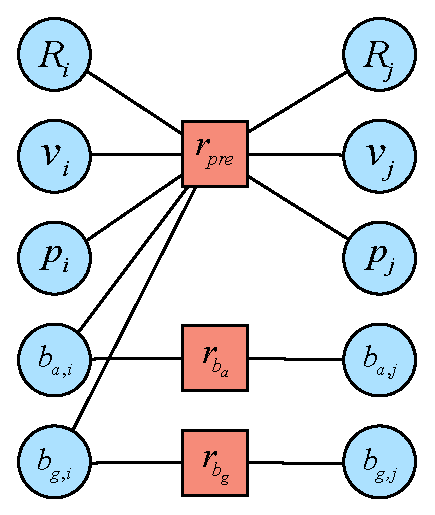
\includegraphics[width=0.4\textwidth]{resources/preintegration/preintegration-residual-graph.pdf}
	\caption{Graph optimization form of the preintegration factor}
	\label{fig:preintegration-residual-graph}
\end{figure}

Apart from placing all state variables in the same vertex, we can also choose a "disassembled form," where rotation, translation, linear velocity, and the two biases are each constructed as separate vertices, and then the Jacobians between these vertices are computed. If this approach is adopted, the number of Jacobian matrices will increase, but the dimensionality of individual Jacobians can be reduced (single Jacobians are typically $3 \times 3$, while the Jacobian of preintegration observations with respect to state variables becomes $9 \times 15$, with many zero blocks). Moreover, if we need to implement a tightly coupled visual or LiDAR system, since visual and LiDAR observation constraints are usually only related to $\bm{R}, \bm{t}$, some zero blocks in the Jacobian matrices can be avoided. In summary, both approaches have their merits. The code implementation in this book adopts the disassembled approach, where each state variable is written as a separate vertex to constrain them individually.

\subsection{Jacobians of Preintegration}  
\label{sec:preinteg-jacobians}  
Finally, we discuss the Jacobian matrices of preintegration with respect to the state variables. Since the preintegration measurements already summarize the IMU readings over a short period, the derivation of the residuals' Jacobians relative to the state variables becomes straightforward. Below, we derive them.  

First, consider rotation. Rotation depends on $\bm{R}_{i}$, $\bm{R}_j$, and $\bm{b}_{g,i}$. We derive it using the right perturbation on $\mathrm{SO}(3)$:  
\begin{equation}\label{key}  
	\begin{aligned}  
		\bm{r}_{\Delta \bm{R}_{ij}}\left(\bm{R}_i \mathrm{Exp} (\boldsymbol{\phi}_i)\right) &=   
		\mathrm{Log} \left( \Delta \tilde{\bm{R}}_{ij}^\top ((\bm{R}_i   
		\mathrm{Exp}(\boldsymbol{\phi_i}))^\top \bm{R}_j \right), \\  
		&= \mathrm{Log} \left( \Delta \tilde{\bm{R}}_{ij}^\top \mathrm{Exp} (-\boldsymbol{\phi}_i )   
		\bm{R}_i^\top \bm{R}_j \right), \\  
		&= \mathrm{Log} \left( \Delta \tilde{\bm{R}}_{ij}^\top \bm{R}_i^\top \bm{R}_j   
		\mathrm{Exp} (-\bm{R}_j^\top \bm{R}_i \boldsymbol{\phi}_i) \right), \\  
		&= \bm{r}_{\Delta \bm{R}_{ij}} - \bm{J}_r^{-1} (\bm{r}_{\Delta \bm{R}_{ij}}) \bm{R}_j^\top   
		\bm{R}_i \boldsymbol{\phi}_i.  
	\end{aligned}  
\end{equation}  

The derivative with respect to $\boldsymbol{\phi}_j$ is:  
\begin{equation}\label{key}  
	\begin{aligned}  
		\bm{r}_{\Delta \bm{R}_{ij}} (\bm{R}_j \mathrm{Exp}(\boldsymbol{\phi}_j)) &=   
		\mathrm{Log}\left(\Delta \tilde{\bm{R}}_{ij}^\top \bm{R}^\top_i \bm{R}_j   
		\mathrm{Exp} (\boldsymbol{\phi}_j ) \right), \\  
		&= \bm{r}_{\Delta \bm{R}_{ij}} + \bm{J}_r^{-1} (\bm{r}_{\Delta \bm{R}_{ij}}) \boldsymbol{\phi}_j.  
	\end{aligned}  
\end{equation}  

These derivations closely resemble those in pose graphs. However, dealing with the bias terms is slightly more involved. Note that during optimization, the bias terms are continuously updated, and each update uses \eqref{eq:update-bias} to correct the preintegration measurements. Since this process is iterative, we always have an initial measurement and a corrected measurement,  which must be taken into account during the derivation.

\subsection{Jacobians of Preintegration}
\label{sec:preinteg-jacobians}
Assume the initial bias for optimization is $\bm{b}_{g,i}$. At a certain iteration step, the current estimated bias correction is $\delta \bm{b}_{g,i}$, and the corrected preintegrated rotation measurement is $\Delta \tilde{\bm{R}}_{ij}^\prime = \Delta \tilde{\bm{R}}_{ij}(\bm{b}_{g,i} + \delta \bm{b}_{g,i})$, with the residual being $\bm{r}_{\Delta \bm{R}_{ij}}^\prime$. To compute the derivative, we further add $\tilde{\delta} \bm{b}_{g,i}$ to these two terms, yielding:

\begin{equation}\label{key}
	\small
	\begin{aligned}
		\bm{r}_{\Delta \bm{R}_{ij}} (\bm{b}_{g,i} + \delta \bm{b}_{g,i} + \tilde{\delta} \bm{b}_{g,i}) &= 
		\mathrm{Log}\left( \left( \Delta \tilde{\bm{R}}_{ij} \mathrm{Exp} \left( \frac{\partial \Delta 
			\tilde{\bm{R}}_{ij}}{\partial \bm{b}_{g,i}} (\delta \bm{b}_{g,i} + \tilde{\delta} \bm{b}_{g,i}) \right) 
		\right)^\top \bm{R}_i^\top \bm{R}_j \right), \\
		&\buildrel\text{BCH}\over\approx \mathrm{Log} \left( \left( \underbrace{\Delta \tilde{\bm{R}}_{ij} 
			\mathrm{Exp} (\frac{\partial \Delta \tilde{\bm{R}}_{ij}}{\partial \bm{b}_{g,i}} \delta 
			\bm{b}_{g,i})}_{\Delta \tilde{\bm{R}}_{ij}^\prime} \mathrm{Exp} (\bm{J}_{r, b} \frac{\partial \Delta 
			\tilde{\bm{R}}_{ij}}{\partial \bm{b}_{g,i}} \tilde{\delta} \bm{b}_{g,i}) \right)^\top 
		\bm{R}_i^\top \bm{R}_j \right), \\
		&= \mathrm{Log} \left( \mathrm{Exp} \left(-\bm{J}_{r,b} \frac{\partial \Delta 
			\tilde{\bm{R}}_{ij}}{\partial \bm{b}_{g,i}} \tilde{\delta} \bm{b}_{g,i} \right) \underbrace{(\Delta 
			\tilde{\bm{R}}_{ij}^\prime)^\top \bm{R}_i^\top \bm{R}_j}_{ \mathrm{Exp} \left( 
			\bm{r}_{ \Delta \bm{R}_{ij}}^\prime \right)} \right), \\
		&= \mathrm{Log} \left( \mathrm{Exp} \left(\bm{r}_{\Delta \bm{R}_{ij}}^\prime \right) \mathrm{Exp} 
		\left( - \mathrm{Exp}\left(\bm{r}_{\Delta \bm{R}_{ij}}^\prime \right)^\top \bm{J}_{r,b} 
		\frac{\partial \Delta \tilde{\bm{R}}_{ij}}{\partial \bm{b}_{g,i}} \tilde{\delta} \bm{b}_{g,i} \right)  \right), \\
		&\approx \bm{r}_{\Delta \bm{R}_{ij}}^\prime - \bm{J}_r^{-1} (\bm{r}_{\Delta \bm{R}_{ij}}^\prime ) 
		\mathrm{Exp}\left(\bm{r}_{\Delta \bm{R}_{ij}}^\prime \right)^\top \bm{J}_{r,b} \frac{\partial 
			\Delta \tilde{\bm{R}}_{ij}}{\partial \bm{b}_{g,i}} \tilde{\delta} \bm{b}_{g,i} .
	\end{aligned}
\end{equation}

Thus, we finally obtain:
\begin{equation}\label{key}
	\frac{\partial \bm{r}_{\Delta \bm{R}_{ij}}}{\partial \bm{b}_{g,i}} = - \bm{J}_r^{-1} (\bm{r}_{\Delta 
		\bm{R}_{ij}}^\prime ) \mathrm{Exp}\left(\bm{r}_{\Delta \bm{R}_{ij}}^\prime \right)^\top 
	\bm{J}_{r,b} \frac{\partial \Delta \tilde{\bm{R}}_{ij}}{\partial \bm{b}_{g,i}}.
\end{equation}

Next, consider the Jacobians for the velocity term. The velocity term is simpler, as it has a linear relationship with $\bm{v}_i$ and $\bm{v}_j$, yielding:
\begin{subequations}\label{key}
	\begin{align}
		\frac{ \partial \bm{r}_{\Delta \bm{v}_{ij}}}{\partial \bm{v}_i} &= -\bm{R}_i^\top, \\
		\frac{ \partial \bm{r}_{\Delta \bm{v}_{ij}}}{\partial \bm{v}_j} &= \bm{R}_i^\top.
	\end{align}
\end{subequations}

For the rotation part, a first-order Taylor expansion suffices:
\begin{equation}
	\begin{aligned}
		\bm{r}_{\Delta \bm{v}_{ij}} \left( \bm{R}_i \mathrm{Exp} (\delta \boldsymbol{\phi}_i)\right) &= 
		(\bm{R}_i \mathrm{Exp} (\delta \boldsymbol{\phi}_i)) ^\top (\bm{v}_j - \bm{v}_i - \bm{g} \Delta 
		t_{ij}) - \Delta \tilde{\bm{v}}_{ij}, \\
		&= (\bm{I} - \delta \boldsymbol{\phi}^\wedge_i) \bm{R}_i^\top  (\bm{v}_j - \bm{v}_i - \bm{g} 
		\Delta t_{ij}) - \Delta \tilde{\bm{v}}_{ij}, \\
		&= \bm{r}_{\Delta \bm{v}_{ij}} (\bm{R}_i) + \left(\bm{R}_i^\top  (\bm{v}_j - \bm{v}_i - \bm{g} 
		\Delta t_{ij}) \right)^\mathrm{\wedge} \delta \boldsymbol{\phi}_i.
	\end{aligned}
\end{equation}

The Jacobians of the velocity residual with respect to $\bm{b}_{g,i}$ and $\bm{b}_{a,i}$ depend only on $\Delta \tilde{\bm{v}}_{ij}$. Since the velocity residual term differs from it only by a negative sign, we simply need to add a negative sign to \eqref{eq:preinteg-jacob-bias}.

Finally, consider the translation part. The translation term depends linearly on $\bm{p}_i$, $\bm{p}_j$, $\bm{v}_i$, $\bm{R}_i$, and the two biases, making the Jacobians straightforward to derive:
\begin{subequations}\label{key}
	\begin{align}
		\frac{\partial \bm{r}_{\Delta \bm{p}_{ij}}}{\partial \bm{p}_i } &= -\bm{R}_i^\top, \\
		\frac{\partial \bm{r}_{\Delta \bm{p}_{ij}}}{\partial \bm{p}_j } &= \bm{R}_i^\top, \\
		\frac{\partial \bm{r}_{\Delta \bm{p}_{ij}}}{\partial \bm{v}_i } &= -\bm{R}_i^\top \Delta t_{ij}, \\
		\frac{\partial \bm{r}_{\Delta \bm{p}_{ij}}}{\partial \boldsymbol{\phi}_i } &= \left( 
		\bm{R}_i^\top \left(\bm{p}_j - \bm{p}_i - \bm{v}_i \Delta t_{ij} - \frac{1}{2}\bm{g} \Delta 
		t_{ij}^2 \right) \right)^\wedge.
	\end{align}
\end{subequations}
The residual for the biases simply requires adding a negative sign to Equation \eqref{eq:preinteg-jacob-bias}.

At this point, we have derived the derivative forms of the preintegrated measurements with respect to all state variables. If desired, we could write the preintegrated observations as a column vector, the state variables as another column vector, and combine all these Jacobian matrices accordingly. To save space, this book presents the preintegration matrices in their decomposed form.

\subsection{Summary}
Finally, we summarize the practical implementation process of the aforementioned preintegration in real-world applications.

In a system composed of keyframes, we can initiate the preintegration process starting from any keyframe at any given time and terminate it at any desired moment. Subsequently, we can extract the preintegrated measurements, noise terms, and various accumulated Jacobians to constrain the states between two keyframes. Based on previous discussions, once preintegration begins, whenever a new IMU measurement arrives, our program should perform the following tasks:
\begin{enumerate}
	\item 
	Compute the three \textbf{preintegrated measurements} using Equation \eqref{eq:def-preintegration} based on the previous data: $\Delta \tilde{\bm{R}}_{ij}, \Delta \tilde{\bm{v}}_{ij}, \Delta \tilde{\bm{p}}_{ij}$;
	\item Calculate the \textbf{covariance matrices} of the three noise terms, which will serve as the information matrices for subsequent graph optimization;
	\item Compute the \textbf{Jacobian matrices} of the preintegrated measurements with respect to the biases - five in total;
\end{enumerate}

Upon completion of the preintegration calculations, these results can be extracted and applied during the optimization process.

\section{Practice: Implementation of Preintegration}
\subsection{Implementing the Preintegration Class}

Following the derivations from the previous section, we now implement the preintegration program. The implementation mainly consists of two parts: the computation of preintegration itself, and its integration into graph optimization. The former is relatively simple as it only involves IMU measurements, while the latter depends on the specific graph optimization framework - in this book we'll implement it using the g2o framework.

First, let's implement the preintegration structure itself. A preintegration class should store the following data:
\begin{itemize}
	\item Preintegrated measurements $\Delta \tilde{\bm{R}}_{ij}, \Delta \tilde{\bm{p}}_{ij}, \Delta \tilde{\bm{v}}_{ij}$;
	\item IMU biases at the start of preintegration $\bm{b}_g, \bm{b}_a$;
	\item Measurement noise covariance $\boldsymbol{\Sigma}_{i,k+1}$ during integration, as specified by Equation \eqref{eq:preinteg-motion-noise};
	\item Jacobian matrices of integrated quantities with respect to IMU biases (see Equation \eqref{eq:preinteg-jacob-bias-inc});
	\item Total integration time $\Delta t_{ij}$.
\end{itemize}

The above are all essential information. Additionally, we may choose to store IMU measurements in the preintegration class (though this is optional since they're already integrated). The IMU measurement noise and bias random walk noise can also be included as configuration parameters. Here's the basic implementation of such a preintegration class:

\begin{lstlisting}[language=c++, caption=src/ch4/imu\_preintegration.h]
class IMUPreintegration {
	public:
	/// Other functions omitted
	struct Options {
		Options() {}
		Vec3d init_bg_ = Vec3d::Zero();  // Initial bias
		Vec3d init_ba_ = Vec3d::Zero();  // Initial bias
		double noise_gyro_ = 1e-2;       // Gyro noise (std dev)
		double noise_acce_ = 1e-1;       // Accelerometer noise (std dev)
	};
	
	public:
	double dt_ = 0;                          // Total preintegration time
	Mat9d cov_ = Mat9d::Zero();              // Accumulated noise matrix
	Mat6d noise_gyro_acce_ = Mat6d::Zero();  // Measurement noise matrix
	
	// Biases
	Vec3d bg_ = Vec3d::Zero();
	Vec3d ba_ = Vec3d::Zero();
	
	// Preintegrated measurements
	SO3 dR_;
	Vec3d dv_ = Vec3d::Zero();
	Vec3d dp_ = Vec3d::Zero();
	
	// Jacobian matrices
	Mat3d dR_dbg_ = Mat3d::Zero();
	Mat3d dV_dbg_ = Mat3d::Zero();
	Mat3d dV_dba_ = Mat3d::Zero();
	Mat3d dP_dbg_ = Mat3d::Zero();
	Mat3d dP_dba_ = Mat3d::Zero();
};
\end{lstlisting}

The variables maintained by this class correspond to those introduced earlier. Note that the IMU bias-related noise terms are not directly part of the preintegration class - we'll move them to the optimization class. This class mainly handles the preintegration of IMU data and provides the integrated measurements and noise values.

\section{Practice: Implementation of Preintegration}
\subsection{Implementing the Single IMU Integration}

The implementation of single IMU integration is as follows:
\begin{lstlisting}[language=c++,caption=src/ch4/imu\_preintegration.cc]
void IMUPreintegration::Integrate(const IMU &imu, double dt) {
	// Remove bias from measurements
	Vec3d gyr = imu.gyro_ - bg_;  // Gyroscope
	Vec3d acc = imu.acce_ - ba_;  // Accelerometer
	
	// Update dv, dp, see (4.7)
	dp_ = dp_ + dv_ * dt + 0.5f * dR_.matrix() * acc * dt * dt;
	dv_ = dv_ + dR_ * acc * dt;
	
	// dR update deferred as current dR needed for A, B matrices
	
	// Jacobian coefficients for motion equation, matrices A,B, see (4.29)
	// Other terms handled later
	Eigen::Matrix<double, 9, 9> A;
	A.setIdentity();
	Eigen::Matrix<double, 9, 6> B;
	B.setZero();
	
	Mat3d acc_hat = SO3::hat(acc);
	double dt2 = dt * dt;
	
	// NOTE: Top-left blocks of A, B differ slightly from formula
	A.block<3, 3>(3, 0) = -dR_.matrix() * dt * acc_hat;
	A.block<3, 3>(6, 0) = -0.5f * dR_.matrix() * acc_hat * dt2;
	A.block<3, 3>(6, 3) = dt * Mat3d::Identity();
	
	B.block<3, 3>(3, 3) = dR_.matrix() * dt;
	B.block<3, 3>(6, 3) = 0.5f * dR_.matrix() * dt2;
	
	// Update Jacobians, see (4.39)
	dP_dba_ = dP_dba_ + dV_dba_ * dt - 0.5f * dR_.matrix() * dt2;                      // (4.39d)
	dP_dbg_ = dP_dbg_ + dV_dbg_ * dt - 0.5f * dR_.matrix() * dt2 * acc_hat * dR_dbg_;  // (4.39e)
	dV_dba_ = dV_dba_ - dR_.matrix() * dt;                                             // (4.39b)
	dV_dbg_ = dV_dbg_ - dR_.matrix() * dt * acc_hat * dR_dbg_;                         // (4.39c)
	
	// Rotation part
	Vec3d omega = gyr * dt;         // Rotation amount
	Mat3d rightJ = SO3::jr(omega);  // Right Jacobian
	SO3 deltaR = SO3::exp(omega);   // After exp
	dR_ = dR_ * deltaR;             // (4.7a)
	
	A.block<3, 3>(0, 0) = deltaR.matrix().transpose();
	B.block<3, 3>(0, 0) = rightJ * dt;
	
	// Update noise term
	cov_ = A * cov_ * A.transpose() + B * noise_gyro_acce_ * B.transpose();
	
	// Update dR_dbg
	dR_dbg_ = deltaR.matrix().transpose() * dR_dbg_ - rightJ * dt;  // (4.39a)
	
	// Increment integration time
	dt_ += dt;
}
\end{lstlisting}

We've added equation numbers in the code comments to help readers locate corresponding formulas. Overall, it updates internal member variables in the following order:
\begin{enumerate}
	\item Updates position and velocity measurements;
	\item Updates noise matrix for motion model;
	\item Updates Jacobians of measurements with respect to biases;
	\item Updates rotation measurements;
	\item Updates integration time.
\end{enumerate}

This completes one IMU data operation. Note that without optimization, preintegration and direct integration produce identical results - both integrate IMU data. After preintegration, we can predict from initial to final state similar to ESKF. The prediction function is straightforward:

\begin{lstlisting}[language=c++,caption=src/ch4/imu\_preintegraion.cc]
NavStated IMUPreintegration::Predict(const sad::NavStated &start, const Vec3d &grav) {
	SO3 Rj = start.R_ * dR_;
	Vec3d vj = start.R_ * dv_ + start.v_ + grav * dt_;
	Vec3d pj = start.R_ * dp_ + start.p_ + start.v_ * dt_ + 0.5f * grav * dt_ * dt_;
	
	auto state = NavStated(start.timestamp_ + dt_, Rj, pj, vj);
	state.bg_ = bg_;
	state.ba_ = ba_;
	return state;
}
\end{lstlisting}

Unlike ESKF, preintegration can predict multiple IMU measurements and predict forward from any starting time, while ESKF typically only predicts from current state to next timestamp for single IMU measurement.

Next, we write a test program to verify whether there is a significant difference between preintegration and direct integration when a constant angular velocity and acceleration are present in a single direction. This method is very effective for identifying obvious errors in the code. Since we implemented the ESKF in the previous chapter, we can also compare the prediction process of ESKF with preintegration. If the initial states are the same, the results should be completely consistent.

\begin{lstlisting}[language=c++,caption=src/ch4/test\_preintegraion.cc]
TEST(PREINTEGRATION_TEST, ROTATION_TEST) {
	// Test the case of preintegration under constant angular velocity
	double imu_time_span = 0.01;       // IMU measurement interval
	Vec3d constant_omega(0, 0, M_PI);  // Angular velocity of 180 deg/s, rotating for 1 second equals 180 degrees
	Vec3d gravity(0, 0, -9.8);         // Z is upward, gravity is in the negative direction
	
	sad::NavStated start_status(0), end_status(1.0);
	sad::IMUPreintegration pre_integ;
	
	// Compare with direct integration
	Sophus::SO3d R;
	Vec3d t = Vec3d::Zero();
	Vec3d v = Vec3d::Zero();
	
	for (int i = 1; i <= 100; ++i) {
		double time = imu_time_span * i;
		Vec3d acce = -gravity;  // Accelerometer should measure an upward force
		pre_integ.Integrate(sad::IMU(time, constant_omega, acce), imu_time_span);
		
		sad::NavStated this_status = pre_integ.Predict(start_status, gravity);
		
		t = t + v * imu_time_span + 0.5 * gravity * imu_time_span * imu_time_span +
		0.5 * (R * acce) * imu_time_span * imu_time_span;
		v = v + gravity * imu_time_span + (R * acce) * imu_time_span;
		R = R * Sophus::SO3d::exp(constant_omega * imu_time_span);
		
		// Verify that under simple conditions, direct integration and preintegration yield the same result
		EXPECT_NEAR(t[0], this_status.p_[0], 1e-2);
		EXPECT_NEAR(t[1], this_status.p_[1], 1e-2);
		EXPECT_NEAR(t[2], this_status.p_[2], 1e-2);
		
		EXPECT_NEAR(v[0], this_status.v_[0], 1e-2);
		EXPECT_NEAR(v[1], this_status.v_[1], 1e-2);
		EXPECT_NEAR(v[2], this_status.v_[2], 1e-2);
		
		EXPECT_NEAR(R.unit_quaternion().x(), this_status.R_.unit_quaternion().x(), 1e-4);
		EXPECT_NEAR(R.unit_quaternion().y(), this_status.R_.unit_quaternion().y(), 1e-4);
		EXPECT_NEAR(R.unit_quaternion().z(), this_status.R_.unit_quaternion().z(), 1e-4);
		EXPECT_NEAR(R.unit_quaternion().w(), this_status.R_.unit_quaternion().w(), 1e-4);
	}
	
	end_status = pre_integ.Predict(start_status);
	
	LOG(INFO) << "preinteg result: ";
	LOG(INFO) << "end rotation: \n" << end_status.R_.matrix();
	LOG(INFO) << "end trans: \n" << end_status.p_.transpose();
	LOG(INFO) << "end v: \n" << end_status.v_.transpose();
	
	LOG(INFO) << "direct integ result: ";
	LOG(INFO) << "end rotation: \n" << R.matrix();
	LOG(INFO) << "end trans: \n" << t.transpose();
	LOG(INFO) << "end v: \n" << v.transpose();
	SUCCEED();
}
\end{lstlisting}

This code uses the gtest framework to verify whether there is a significant difference between IMU integration and preintegration under a fixed angular velocity measurement along the $Z$ axis. The same file also contains tests for constant acceleration and comparisons with ESKF. Since the code is very similar, we do not list it here. Readers can run this code to check whether the IMU operations in the preintegration module are implemented correctly.

\subsection{Graph Optimization Vertices for Pre-integration}

Next, we will implement the graph optimization related to pre-integration. Compared to the filter framework, the graph optimization framework is slightly more complex but offers greater flexibility in usage. We will introduce the variables and classes related to graph optimization one by one.

First, our 15-dimensional or 18-dimensional state variables should correspond to the vertices in graph optimization. They use generalized addition to implement operations on matrix manifolds and tangent spaces. This book adopts a \textbf{bulk} form, so each state is divided into four types of vertices: pose, velocity, gyroscope bias, and accelerometer bias. The latter three are essentially variables in $\mathbb{R}^3$ and can be directly implemented using inheritance.

\begin{lstlisting}[language=c++,caption=src/common/g2o\_types.h]
class VertexPose : public g2o::BaseVertex<6, SE3> {
	public:
	EIGEN_MAKE_ALIGNED_OPERATOR_NEW
	VertexPose() {}
	
	virtual void oplusImpl(const double* update_) {
		_estimate.so3() = _estimate.so3() * SO3::exp(Eigen::Map<const Vec3d>(&update_[0]));  // Rotation part
		_estimate.translation() += Eigen::Map<const Vec3d>(&update_[3]);                     // Translation part
		updateCache();
	}
};

/**
* Velocity vertex, simply Vec3d
*/
class VertexVelocity : public g2o::BaseVertex<3, Vec3d> {
	public:
	VertexVelocity() {}
	virtual void oplusImpl(const double* update_) {
		Vec3d uv;
		uv << update_[0], update_[1], update_[2];
		setEstimate(estimate() + uv);
	}
};

/**
* Gyroscope bias vertex, also Vec3d, inherits from velocity vertex
*/
class VertexGyroBias : public VertexVelocity {
	public:
	VertexGyroBias() {}
};

/**
* Accelerometer bias vertex, Vec3d, also inherits from velocity vertex
*/
class VertexAccBias : public VertexVelocity {
	public:
	VertexAccBias() {}
};
\end{lstlisting}

We have only listed the key implementation parts, omitting some default constructors. We combine rotation and translation in the same VertexPose vertex. Special attention should be paid to the variable ordering here. Inside VertexPose, rotation comes first followed by translation, so the Jacobian matrix ordering must correspond accordingly.

\subsection{Graph Optimization Edges for Pre-integration Scheme}

Next, we will formulate the prediction and update equations from the previous chapter's GINS system into graph optimization form. Let's summarize the optimization-related edges as follows:
\begin{enumerate}
	\item Pre-integration edges, which constrain the 15-dimensional state from the previous timestamp to the rotation, translation, and velocity at the next timestamp;
	\item Bias random walk edges (two types), connecting bias states between two timestamps;
	\item GNSS observation edges. Since we use 6-DOF observations, they associate with the pose at a single timestamp;
	\item Prior information, characterizing the state distribution at the previous timestamp and associating with the 15-dimensional state at that time;
	\item Wheel odometer observation edges, associating with the velocity vertex at the previous timestamp.
\end{enumerate}

We will implement these components sequentially. First is the most complex pre-integration edge. Its error function and Jacobian function are as follows:
\begin{lstlisting}[language=c++,caption=src/ch4/g2o\_types.cc]
class EdgeInertial : public g2o::BaseMultiEdge<9, Vec9d> {
	public:
	EIGEN_MAKE_ALIGNED_OPERATOR_NEW
	
	/**
	* The constructor needs to specify the pre-integration class object
	* @param preinteg   Pointer to the pre-integration object
	* @param gravity    Gravity vector
	* @param weight     Weight
	*/
	EdgeInertial(std::shared_ptr<IMUPreintegration> preinteg, const Vec3d& gravity, double weight = 1.0);
	
	void computeError() override;
	void linearizeOplus() override;
	private:
	const double dt_;
	std::shared_ptr<IMUPreintegration> preint_ = nullptr;
	Vec3d grav_;
};

EdgeInertial::EdgeInertial(std::shared_ptr<IMUPreintegration> preinteg, const Vec3d& gravity, double weight)
: preint_(preinteg), dt_(preinteg->dt_) {
	resize(6);  // 6 connected vertices
	grav_ = gravity;
	setInformation(preinteg->cov_.inverse() * weight);
}

void EdgeInertial::computeError() {
	auto* p1 = dynamic_cast<const VertexPose*>(_vertices[0]);
	auto* v1 = dynamic_cast<const VertexVelocity*>(_vertices[1]);
	auto* bg1 = dynamic_cast<const VertexGyroBias*>(_vertices[2]);
	auto* ba1 = dynamic_cast<const VertexAccBias*>(_vertices[3]);
	auto* p2 = dynamic_cast<const VertexPose*>(_vertices[4]);
	auto* v2 = dynamic_cast<const VertexVelocity*>(_vertices[5]);
	
	Vec3d bg = bg1->estimate();
	Vec3d ba = ba1->estimate();
	
	const SO3 dR = preint_->GetDeltaRotation(bg);
	const Vec3d dv = preint_->GetDeltaVelocity(bg, ba);
	const Vec3d dp = preint_->GetDeltaPosition(bg, ba);
	
	/// Pre-integration error terms (4.41)
	const Vec3d er = (dR.inverse() * p1->estimate().so3().inverse() * p2->estimate().so3()).log();
	Mat3d RiT = p1->estimate().so3().inverse().matrix();
	const Vec3d ev = RiT * (v2->estimate() - v1->estimate() - grav_ * dt_) - dv;
	const Vec3d ep = RiT * (p2->estimate().translation() - p1->estimate().translation() - v1->estimate() * dt_ -
	grav_ * dt_ * dt_ / 2) -
	dp;
	_error << er, ev, ep;
}

void EdgeInertial::linearizeOplus() {
	auto* p1 = dynamic_cast<const VertexPose*>(_vertices[0]);
	auto* v1 = dynamic_cast<const VertexVelocity*>(_vertices[1]);
	auto* bg1 = dynamic_cast<const VertexGyroBias*>(_vertices[2]);
	auto* ba1 = dynamic_cast<const VertexAccBias*>(_vertices[3]);
	auto* p2 = dynamic_cast<const VertexPose*>(_vertices[4]);
	auto* v2 = dynamic_cast<const VertexVelocity*>(_vertices[5]);
	
	Vec3d bg = bg1->estimate();
	Vec3d ba = ba1->estimate();
	Vec3d dbg = bg - preint_->bg_;
	
	// Intermediate symbols
	const SO3 R1 = p1->estimate().so3();
	const SO3 R1T = R1.inverse();
	const SO3 R2 = p2->estimate().so3();
	
	auto dR_dbg = preint_->dR_dbg_;
	auto dv_dbg = preint_->dV_dbg_;
	auto dp_dbg = preint_->dP_dbg_;
	auto dv_dba = preint_->dV_dba_;
	auto dp_dba = preint_->dP_dba_;
	
	// Estimates
	Vec3d vi = v1->estimate();
	Vec3d vj = v2->estimate();
	Vec3d pi = p1->estimate().translation();
	Vec3d pj = p2->estimate().translation();
	
	const SO3 dR = preint_->GetDeltaRotation(bg);
	const SO3 eR = SO3(dR).inverse() * R1T * R2;
	const Vec3d er = eR.log();
	const Mat3d invJr = SO3::jr_inv(eR);
	
	/// Jacobian matrices
	/// Note there are 3 indices: vertex index, own error row, and vertex internal variable column
	/// Variable order: pose1(R1,p1), v1, bg1, ba1, pose2(R2,p2), v2
	/// Residual order: eR, ev, ep, with residual order as rows and variable order as columns
	
	//       | R1 | p1 | v1 | bg1 | ba1 | R2 | p2 | v2 |
	//  vert | 0       | 1  | 2   | 3   | 4       | 5  |
	//  col  | 0    3  | 0  | 0   | 0   | 0    3  | 0  |
	//    row
	//  eR 0 |
	//  ev 3 |
	//  ep 6 |
	
	/// Residual w.r.t R1, 9x3
	_jacobianOplus[0].setZero();
	// dR/dR1, 4.42
	_jacobianOplus[0].block<3, 3>(0, 0) = -invJr * (R2.inverse() * R1).matrix();
	// dv/dR1, 4.47
	_jacobianOplus[0].block<3, 3>(3, 0) = SO3::hat(R1T * (vj - vi - grav_ * dt_));
	// dp/dR1, 4.48d
	_jacobianOplus[0].block<3, 3>(6, 0) = SO3::hat(R1T * (pj - pi - v1->estimate() * dt_ - 0.5 * grav_ * dt_ * dt_));
	
	/// Residual w.r.t p1, 9x3
	// dp/dp1, 4.48a
	_jacobianOplus[0].block<3, 3>(6, 3) = -R1T.matrix();
	
	/// Residual w.r.t v1, 9x3
	_jacobianOplus[1].setZero();
	// dv/dv1, 4.46a
	_jacobianOplus[1].block<3, 3>(3, 0) = -R1T.matrix();
	// dp/dv1, 4.48c
	_jacobianOplus[1].block<3, 3>(6, 0) = -R1T.matrix() * dt_;
	
	/// Residual w.r.t bg1
	_jacobianOplus[2].setZero();
	// dR/dbg1, 4.45
	_jacobianOplus[2].block<3, 3>(0, 0) = -invJr * eR.inverse().matrix() * SO3::jr((dR_dbg * dbg).eval()) * dR_dbg;
	// dv/dbg1
	_jacobianOplus[2].block<3, 3>(3, 0) = -dv_dbg;
	// dp/dbg1
	_jacobianOplus[2].block<3, 3>(6, 0) = -dp_dbg;
	
	/// Residual w.r.t ba1
	_jacobianOplus[3].setZero();
	// dv/dba1
	_jacobianOplus[3].block<3, 3>(3, 0) = -dv_dba;
	// dp/dba1
	_jacobianOplus[3].block<3, 3>(6, 0) = -dp_dba;
	
	/// Residual w.r.t pose2
	_jacobianOplus[4].setZero();
	// dr/dr2, 4.43
	_jacobianOplus[4].block<3, 3>(0, 0) = invJr;
	// dp/dp2, 4.48b
	_jacobianOplus[4].block<3, 3>(6, 3) = R1T.matrix();
	
	/// Residual w.r.t v2
	_jacobianOplus[5].setZero();
	// dv/dv2, 4,46b
	_jacobianOplus[5].block<3, 3>(3, 0) = R1T.matrix();  // OK
}
\end{lstlisting}

We have also provided corresponding formulas in the comments for readers to compare. During implementation, we must be careful with the order of Jacobian matrices here. They actually have three indices: \textbf{which vertex}, the \textbf{row of the error term}, and the \textbf{column of the vertex's internal variables}. For example, if we want to compute the Jacobian block of the pre-integration $\Delta \tilde{\bm{p}}_{ij}$ with respect to the translation part of the second pose, i.e., $\bm{p}_j$, then the corresponding Jacobian block should be located at the 4th vertex, 6th row, and 3rd column. Here, the 4th vertex means the pose vertex at time $j$ is the 4th vertex of the pre-integration edge, the 6th row means $\delta \tilde{\bm{p}}_{ij}$ is the 6th row in the pre-integration observation, and the 3rd column means $\bm{p}_j$ is the 3rd column in VertexPose. Regardless of which optimization framework we use, when defining Jacobian matrices ourselves, we will encounter such matrix block ordering issues when dealing with connections between multiple vertices. This is an error-prone area.

Now let's define the edges for biases, GNSS, prior states, and odometry. The two bias edges are essentially identical, so we'll only show one:

\begin{lstlisting}[language=c++,caption=src/common/g2o\_types.h]
class EdgeGyroRW : public g2o::BaseBinaryEdge<3, Vec3d, VertexGyroBias, VertexGyroBias> {
	public:	
	void computeError() {
		const VertexGyroBias* VG1 = static_cast<const VertexGyroBias*>(_vertices[0]);
		const VertexGyroBias* VG2 = static_cast<const VertexGyroBias*>(_vertices[1]);
		_error = VG2->estimate() - VG1->estimate();
	}
	
	virtual void linearizeOplus() {
		_jacobianOplusXi = -Mat3d::Identity();
		_jacobianOplusXj.setIdentity();
	}
};

/**
* Prior for previous frame's IMU pvq bias
* info is specified externally, given by marginalization in time window
*
* Vertex order: pose, v, bg, ba
* Residual order: R, p, v, bg, ba, 15-dimensional
*/
class EdgePriorPoseNavState : public g2o::BaseMultiEdge<15, Vec15d> {
	public:
	void computeError();
	virtual void linearizeOplus();
	NavStated state_;
};

void EdgePriorPoseNavState::computeError() {
	auto* vp = dynamic_cast<const VertexPose*>(_vertices[0]);
	auto* vv = dynamic_cast<const VertexVelocity*>(_vertices[1]);
	auto* vg = dynamic_cast<const VertexGyroBias*>(_vertices[2]);
	auto* va = dynamic_cast<const VertexAccBias*>(_vertices[3]);
	
	const Vec3d er = SO3(state_.R_.matrix().transpose() * vp->estimate().so3().matrix()).log();
	const Vec3d ep = vp->estimate().translation() - state_.p_;
	const Vec3d ev = vv->estimate() - state_.v_;
	const Vec3d ebg = vg->estimate() - state_.bg_;
	const Vec3d eba = va->estimate() - state_.ba_;
	
	_error << er, ep, ev, ebg, eba;
}

void EdgePriorPoseNavState::linearizeOplus() {
	const auto* vp = dynamic_cast<const VertexPose*>(_vertices[0]);
	const Vec3d er = SO3(state_.R_.matrix().transpose() * vp->estimate().so3().matrix()).log();
	
	/// Note there are 3 indices: vertex index, error row, and vertex internal variable column
	_jacobianOplus[0].setZero();
	_jacobianOplus[0].block<3, 3>(0, 0) = SO3::jr_inv(er);    // dr/dr
	_jacobianOplus[0].block<3, 3>(3, 3) = Mat3d::Identity();  // dp/dp
	_jacobianOplus[1].setZero();
	_jacobianOplus[1].block<3, 3>(6, 0) = Mat3d::Identity();  // dv/dv
	_jacobianOplus[2].setZero();
	_jacobianOplus[2].block<3, 3>(9, 0) = Mat3d::Identity();  // dbg/dbg
	_jacobianOplus[3].setZero();
	_jacobianOplus[3].block<3, 3>(12, 0) = Mat3d::Identity();  // dba/dba
}

class EdgeGNSS : public g2o::BaseUnaryEdge<6, SE3, VertexPose> {
	public:
	void computeError() override {
		VertexPose* v = (VertexPose*)_vertices[0];
		_error.head<3>() = (_measurement.so3().inverse() * v->estimate().so3()).log();
		_error.tail<3>() = v->estimate().translation() - _measurement.translation();
	};
	
	void linearizeOplus() override {
		VertexPose* v = (VertexPose*)_vertices[0];
		// jacobian 6x6
		_jacobianOplusXi.setZero();
		_jacobianOplusXi.block<3, 3>(0, 0) = (_measurement.so3().inverse() * v->estimate().so3()).jr_inv();  // dR/dR
		_jacobianOplusXi.block<3, 3>(3, 3) = Mat3d::Identity();                        
	}
};
\end{lstlisting}

Most of the Jacobian matrices here are quite straightforward, and readers should be able to derive them themselves.

\subsection{Implementation of GINS Based on Pre-integration and Graph Optimization}

Finally, we utilize the graph optimization edges defined earlier to implement a GNSS/INS fusion positioning system similar to the ESKF. Readers can also use this experiment to gain deeper insights into the similarities and differences between graph optimization and filter-based approaches. This graph optimization-based GINS system follows essentially the same logic as the ESKF, still requiring static IMU initialization to determine the initial IMU biases and gravity direction. We encapsulate these logical processes in a separate class while focusing on how this graph optimization model is constructed. The basic workflow is as follows:

\begin{enumerate}
	\item 
	We obtain initial biases and gravity direction through an external static IMU initialization algorithm, then use the first GNSS measurement with attitude information to determine the initial position and orientation. When both IMU and GNSS data become available, we begin prediction and optimization.
	
	\item When IMU data arrives, we use the pre-integrator to accumulate IMU integration information.
	
	\item When odometry data arrives, we record it as the most recent velocity observation and retain its readings.
	
	\item When GNSS data arrives, we construct a graph optimization problem between \textbf{the previous timestamp's} GNSS and \textbf{the current timestamp's} GNSS. The nodes and edges of this problem are defined as:
	\begin{itemize}
		\item Nodes: Pose, velocity, and both bias terms (gyro and accelerometer) from the previous and current timestamps - totaling 8 vertices.
		\item Edges: Pre-integration observation edge between two timestamps, GNSS observation edges for both timestamps, prior edge for the previous timestamp, two bias random walk edges, and velocity observation edge - making 7 edges in total.
	\end{itemize}
	
	\item We use the predicted values from IMU pre-integration as initial values for optimization. Alternatively, GNSS observations could also be used for initialization. While these two initialization methods yield different starting points, they produce similar results in our current implementation. Readers are encouraged to experiment with both approaches.
\end{enumerate}

\begin{figure}[!htp]
	\centering
	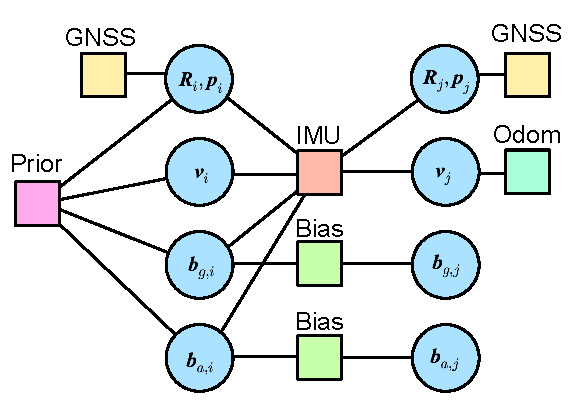
\includegraphics[width=0.5\textwidth]{preintegration/real-factor-graph}
	\caption{Actual graph optimization structure used in the GINS case study}
	\label{fig:real-factor-graph}
\end{figure}

The complete graph optimization structure is shown in Figure~\ref{fig:real-factor-graph}~. We implement GINS as a class that handles IMU, Odom and GNSS observations:

\begin{lstlisting}[language=c++,caption=src/ch4/gins\_pre\_integ.cc]
	void GinsPreInteg::AddImu(const IMU& imu) {
		if (first_gnss_received_ && first_imu_received_) {
			pre_integ_->Integrate(imu, imu.timestamp_ - last_imu_.timestamp_);
		}
		
		first_imu_received_ = true;
		last_imu_ = imu;
		current_time_ = imu.timestamp_;
	}
	
	void GinsPreInteg::AddOdom(const sad::Odom& odom) {
		last_odom_ = odom;
		last_odom_set_ = true;
	}
	
	void GinsPreInteg::AddGnss(const GNSS& gnss) {
		this_frame_ = std::make_shared<NavStated>(current_time_);
		this_gnss_ = gnss;
		
		if (!first_gnss_received_) {
			if (!gnss.heading_valid_) {
				// First GNSS must have valid heading
				return;
			}
			
			// First GNSS measurement sets initial pose
			this_frame_->timestamp_ = gnss.unix_time_;
			this_frame_->p_ = gnss.utm_pose_.translation();
			this_frame_->R_ = gnss.utm_pose_.so3();
			this_frame_->v_.setZero();
			this_frame_->bg_ = options_.preinteg_options_.init_bg_;
			this_frame_->ba_ = options_.preinteg_options_.init_ba_;
			
			pre_integ_ = std::make_shared<IMUPreintegration>(options_.preinteg_options_);
			
			last_frame_ = this_frame_;
			last_gnss_ = this_gnss_;
			first_gnss_received_ = true;
			current_time_ = gnss.unix_time_;
			return;
		}
		
		current_time_ = gnss.unix_time_;
		*this_frame_ = pre_integ_->Predict(*last_frame_, options_.gravity_);
		
		Optimize();
		
		last_frame_ = this_frame_;
		last_gnss_ = this_gnss_;
	}
\end{lstlisting}

The processing functions mainly handle workflow logic, with the key content being the Optimize function:

\begin{lstlisting}[language=c++,caption=src/ch4/gins\_pre\_integ.cc]
	void GinsPreInteg::Optimize() {
		if (pre_integ_->dt_ < 1e-3) {
			// No integration available
			return;
		}
		
		LOG(INFO) << "calling optimization";
		
		using BlockSolverType = g2o::BlockSolverX;
		using LinearSolverType = g2o::LinearSolverEigen<BlockSolverType::PoseMatrixType>;
		
		auto* solver = new g2o::OptimizationAlgorithmLevenberg(
		g2o::make_unique<BlockSolverType>(g2o::make_unique<LinearSolverType>()));
		g2o::SparseOptimizer optimizer;
		optimizer.setAlgorithm(solver);
		
		// Previous timestamp vertices: pose, v, bg, ba
		auto v0_pose = new VertexPose();
		v0_pose->setId(0);
		v0_pose->setEstimate(last_frame_->GetSE3());
		optimizer.addVertex(v0_pose);
		
		auto v0_vel = new VertexVelocity();
		v0_vel->setId(1);
		v0_vel->setEstimate(last_frame_->v_);
		optimizer.addVertex(v0_vel);
		
		auto v0_bg = new VertexGyroBias();
		v0_bg->setId(2);
		v0_bg->setEstimate(last_frame_->bg_);
		optimizer.addVertex(v0_bg);
		
		auto v0_ba = new VertexAccBias();
		v0_ba->setId(3);
		v0_ba->setEstimate(last_frame_->ba_);
		optimizer.addVertex(v0_ba);
		
		// Current timestamp vertices: pose, v, bg, ba
		auto v1_pose = new VertexPose();
		v1_pose->setId(4);
		v1_pose->setEstimate(this_frame_->GetSE3());
		optimizer.addVertex(v1_pose);
		
		auto v1_vel = new VertexVelocity();
		v1_vel->setId(5);
		v1_vel->setEstimate(this_frame_->v_);
		optimizer.addVertex(v1_vel);
		
		auto v1_bg = new VertexGyroBias();
		v1_bg->setId(6);
		v1_bg->setEstimate(this_frame_->bg_);
		optimizer.addVertex(v1_bg);
		
		auto v1_ba = new VertexAccBias();
		v1_ba->setId(7);
		v1_ba->setEstimate(this_frame_->ba_);
		optimizer.addVertex(v1_ba);
		
		// Pre-integration edge
		auto edge_inertial = new EdgeInertial(pre_integ_, options_.gravity_);
		edge_inertial->setVertex(0, v0_pose);
		edge_inertial->setVertex(1, v0_vel);
		edge_inertial->setVertex(2, v0_bg);
		edge_inertial->setVertex(3, v0_ba);
		edge_inertial->setVertex(4, v1_pose);
		edge_inertial->setVertex(5, v1_vel);
		auto* rk = new g2o::RobustKernelHuber();
		rk->setDelta(200.0);
		edge_inertial->setRobustKernel(rk);
		optimizer.addEdge(edge_inertial);
		
		// Bias random walk edges
		auto* edge_gyro_rw = new EdgeGyroRW();
		edge_gyro_rw->setVertex(0, v0_bg);
		edge_gyro_rw->setVertex(1, v1_bg);
		edge_gyro_rw->setInformation(options_.bg_rw_info_);
		optimizer.addEdge(edge_gyro_rw);
		
		auto* edge_acc_rw = new EdgeAccRW();
		edge_acc_rw->setVertex(0, v0_ba);
		edge_acc_rw->setVertex(1, v1_ba);
		edge_acc_rw->setInformation(options_.ba_rw_info_);
		optimizer.addEdge(edge_acc_rw);
		
		// Previous timestamp prior
		auto* edge_prior = new EdgePriorPoseNavState(*last_frame_, prior_info_);
		edge_prior->setVertex(0, v0_pose);
		edge_prior->setVertex(1, v0_vel);
		edge_prior->setVertex(2, v0_bg);
		edge_prior->setVertex(3, v0_ba);
		optimizer.addEdge(edge_prior);
		
		// GNSS edges
		auto edge_gnss0 = new EdgeGNSS(v0_pose, last_gnss_.utm_pose_);
		edge_gnss0->setInformation(options_.gnss_info_);
		optimizer.addEdge(edge_gnss0);
		
		auto edge_gnss1 = new EdgeGNSS(v1_pose, this_gnss_.utm_pose_);
		edge_gnss1->setInformation(options_.gnss_info_);
		optimizer.addEdge(edge_gnss1);
		
		// Odom edge
		EdgeEncoder3D* edge_odom = nullptr;
		Vec3d vel_world = Vec3d::Zero();
		Vec3d vel_odom = Vec3d::Zero();
		if (last_odom_set_) {
			// velocity obs
			double velo_l =
			options_.wheel_radius_ * last_odom_.left_pulse_ / options_.circle_pulse_ * 2 * M_PI / options_.odom_span_;
			double velo_r =
			options_.wheel_radius_ * last_odom_.right_pulse_ / options_.circle_pulse_ * 2 * M_PI / options_.odom_span_;
			double average_vel = 0.5 * (velo_l + velo_r);
			vel_odom = Vec3d(average_vel, 0.0, 0.0);
			vel_world = this_frame_->R_ * vel_odom;
			
			edge_odom = new EdgeEncoder3D(v1_vel, vel_world);
			edge_odom->setInformation(options_.odom_info_);
			optimizer.addEdge(edge_odom);
		}
		
		optimizer.setVerbose(options_.verbose_);
		optimizer.initializeOptimization();
		optimizer.optimize(20);
		
		// Some print functions omitted
		
		// Reset integrator
		options_.preinteg_options_.init_bg_ = this_frame_->bg_;
		options_.preinteg_options_.init_ba_ = this_frame_->ba_;
		pre_integ_ = std::make_shared<IMUPreintegration>(options_.preinteg_options_);
	}
\end{lstlisting}

We have omitted some print information and result retrieval steps. From the code, we can see how the entire optimization model is constructed and solved. This modular vertex approach involves more vertex types and quantities, making implementation slightly more complex. Readers are encouraged to compile and run this program using gflags to specify the input file. The test program source code is similar to the previous chapter and won't be listed again. Execute in terminal:

\begin{lstlisting}[language=sh,caption=Terminal command:]
	bin/run_gins_pre_integ --txt_path ./data/ch3/10.txt 
\end{lstlisting}

\begin{figure}[!htp]
	\centering
	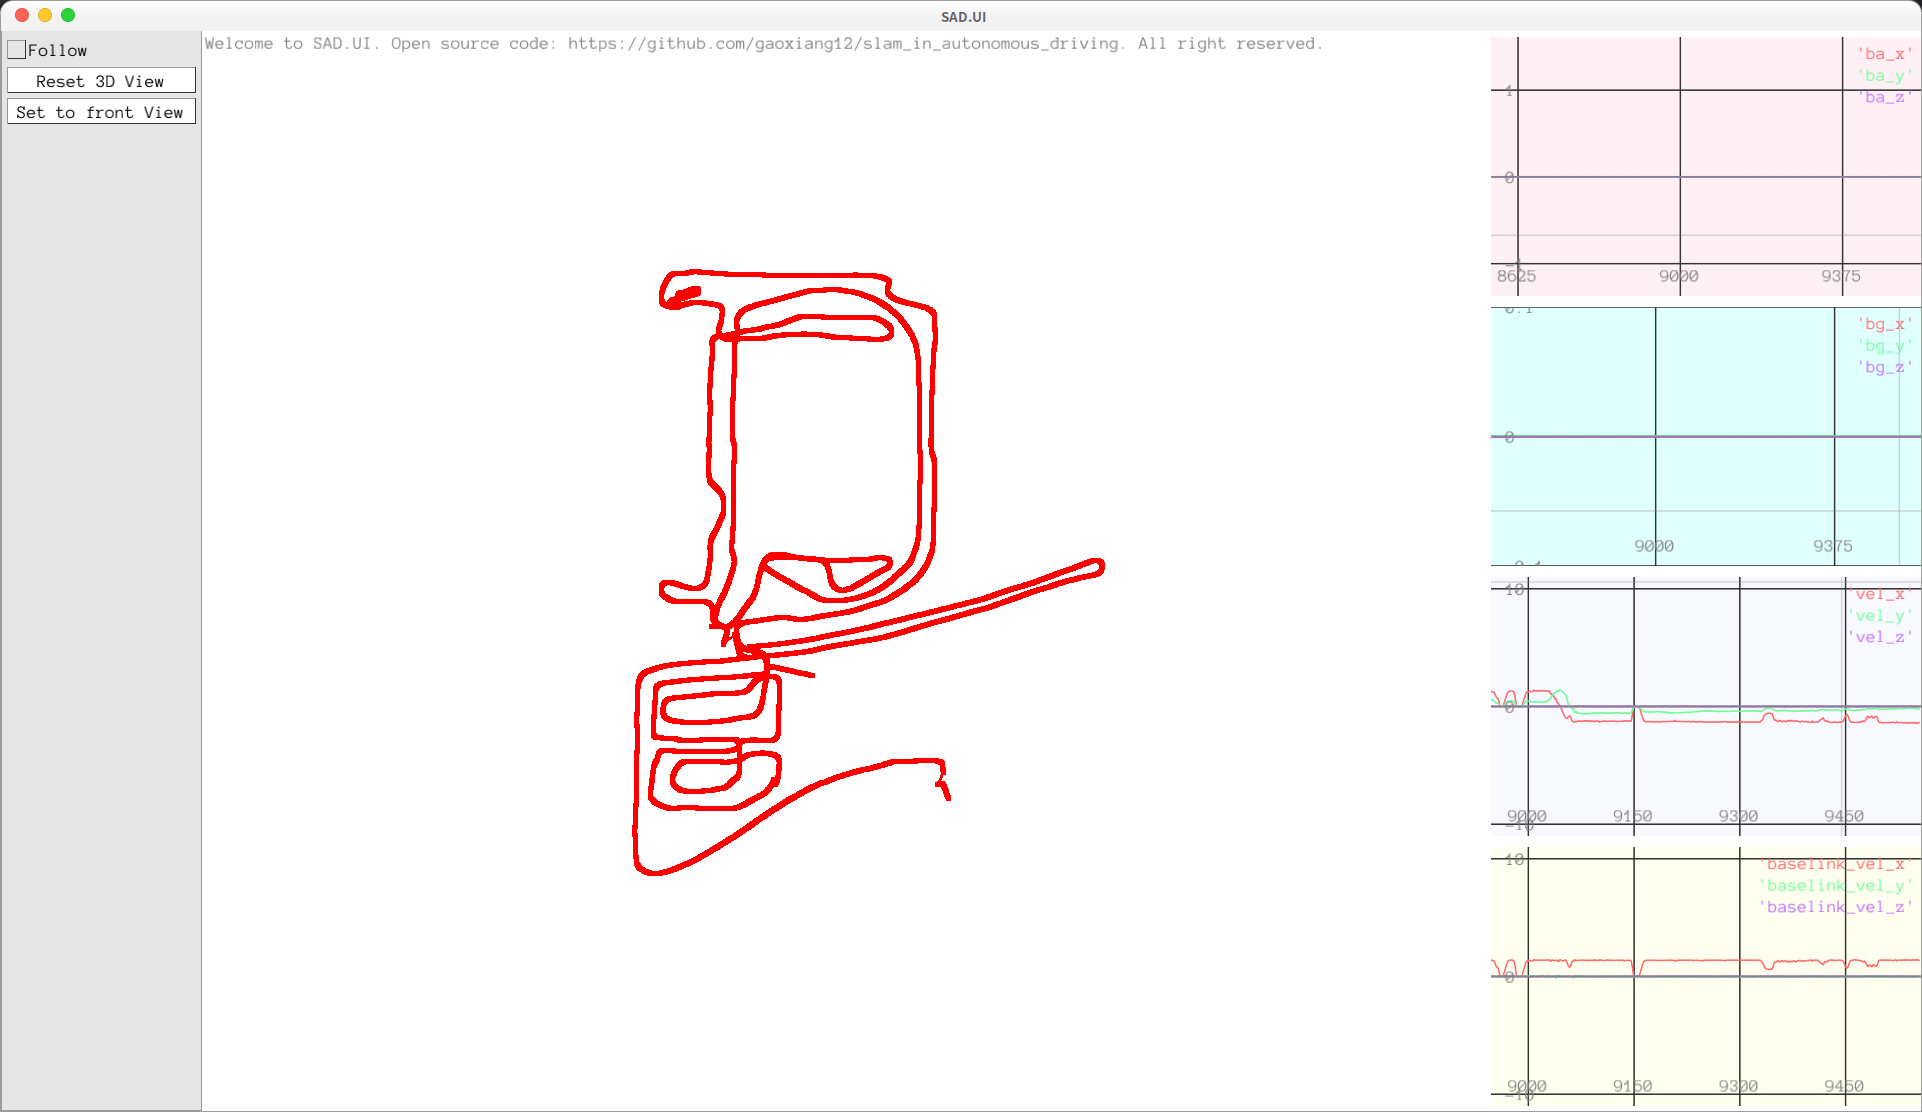
\includegraphics[width=0.8\textwidth]{resources/preintegration/gins-preinteg.png}
	\caption{GINS results based on pre-integration graph optimization}
	\label{fig:gins-preinteg}
\end{figure}

The program will similarly output real-time results and state variable text files. The real-time results are shown in Figure~\ref{fig:gins-preinteg}~, and trajectory results can be plotted using the script from the previous chapter:

\begin{lstlisting}[language=sh,caption=Terminal command:]
	python3 scripts/plot_ch3_state.py ./data/ch4/gins_preintg.txt
\end{lstlisting}

The state diagram is shown in Figure\ref{fig:preintegration-gins}. Overall they are similar to the previous chapter, with velocity states within expected ranges. However, since this chapter's GINS doesn't directly optimize at the Odom level, pure IMU prediction will still diverge locally when GNSS observations are unavailable. Below we discuss the program's approach and its differences from ESKF:

\begin{enumerate}
	\item Compared to ESKF, the pre-integration based graph optimization can accumulate IMU readings. The accumulation duration or number of iterations can be manually selected, while ESKF by default can only iterate once and predict based on single-timestamp IMU data.
	
	\item The pre-integration edge (or called IMU factor/pre-integration factor in factor graph terminology\footnote{This book doesn't distinguish between graph optimization and factor graph concepts, as they are essentially the same in practice. Sometimes we refer to them as \textbf{optimization edges}, other times as \textbf{optimization factors}. Conceptually, \textbf{factor} is more intuitive than \textbf{edge}, so we often discuss various factors while implementing them as edges.}) is a very flexible factor. All six connected vertices can change. To prevent arbitrary state changes, pre-integration factors typically need to be used with other factors. In our case, GNSS factors at both ends constrain pose changes, Odom factors constrain velocity changes, and two bias factors constrain bias variations without limiting absolute bias values.
	
	\item Prior factors make the estimation smoother. Strictly speaking, prior factor covariance matrices should be handled through marginalization. Since this chapter focuses on pre-integration principles, we've set fixed information matrices for prior factors to simplify implementation. In Chapter~\ref{cpt:tightly-lio}~, we'll discuss prior factor information matrix settings and implementation. Readers can try removing this factor to observe its impact on trajectory estimation.
	
	\item Graph optimization conveniently allows setting kernel functions and examining each factor's error contribution, helping identify which parts dominate the optimization. For example, we can analyze normal vs abnormal RTK observation residuals to determine GNSS measurement reliability. Later we'll also introduce how to control optimization flow for more robust results. Readers can enable debug output to examine this information.
	
	\item Due to additional computations, graph optimization is noticeably more time-consuming than filter-based approaches. However, with significant increases in computing power for smart vehicles, graph optimization can now be effectively used in some real-time applications.
\end{enumerate}

\begin{figure}[!t]
	\centering
	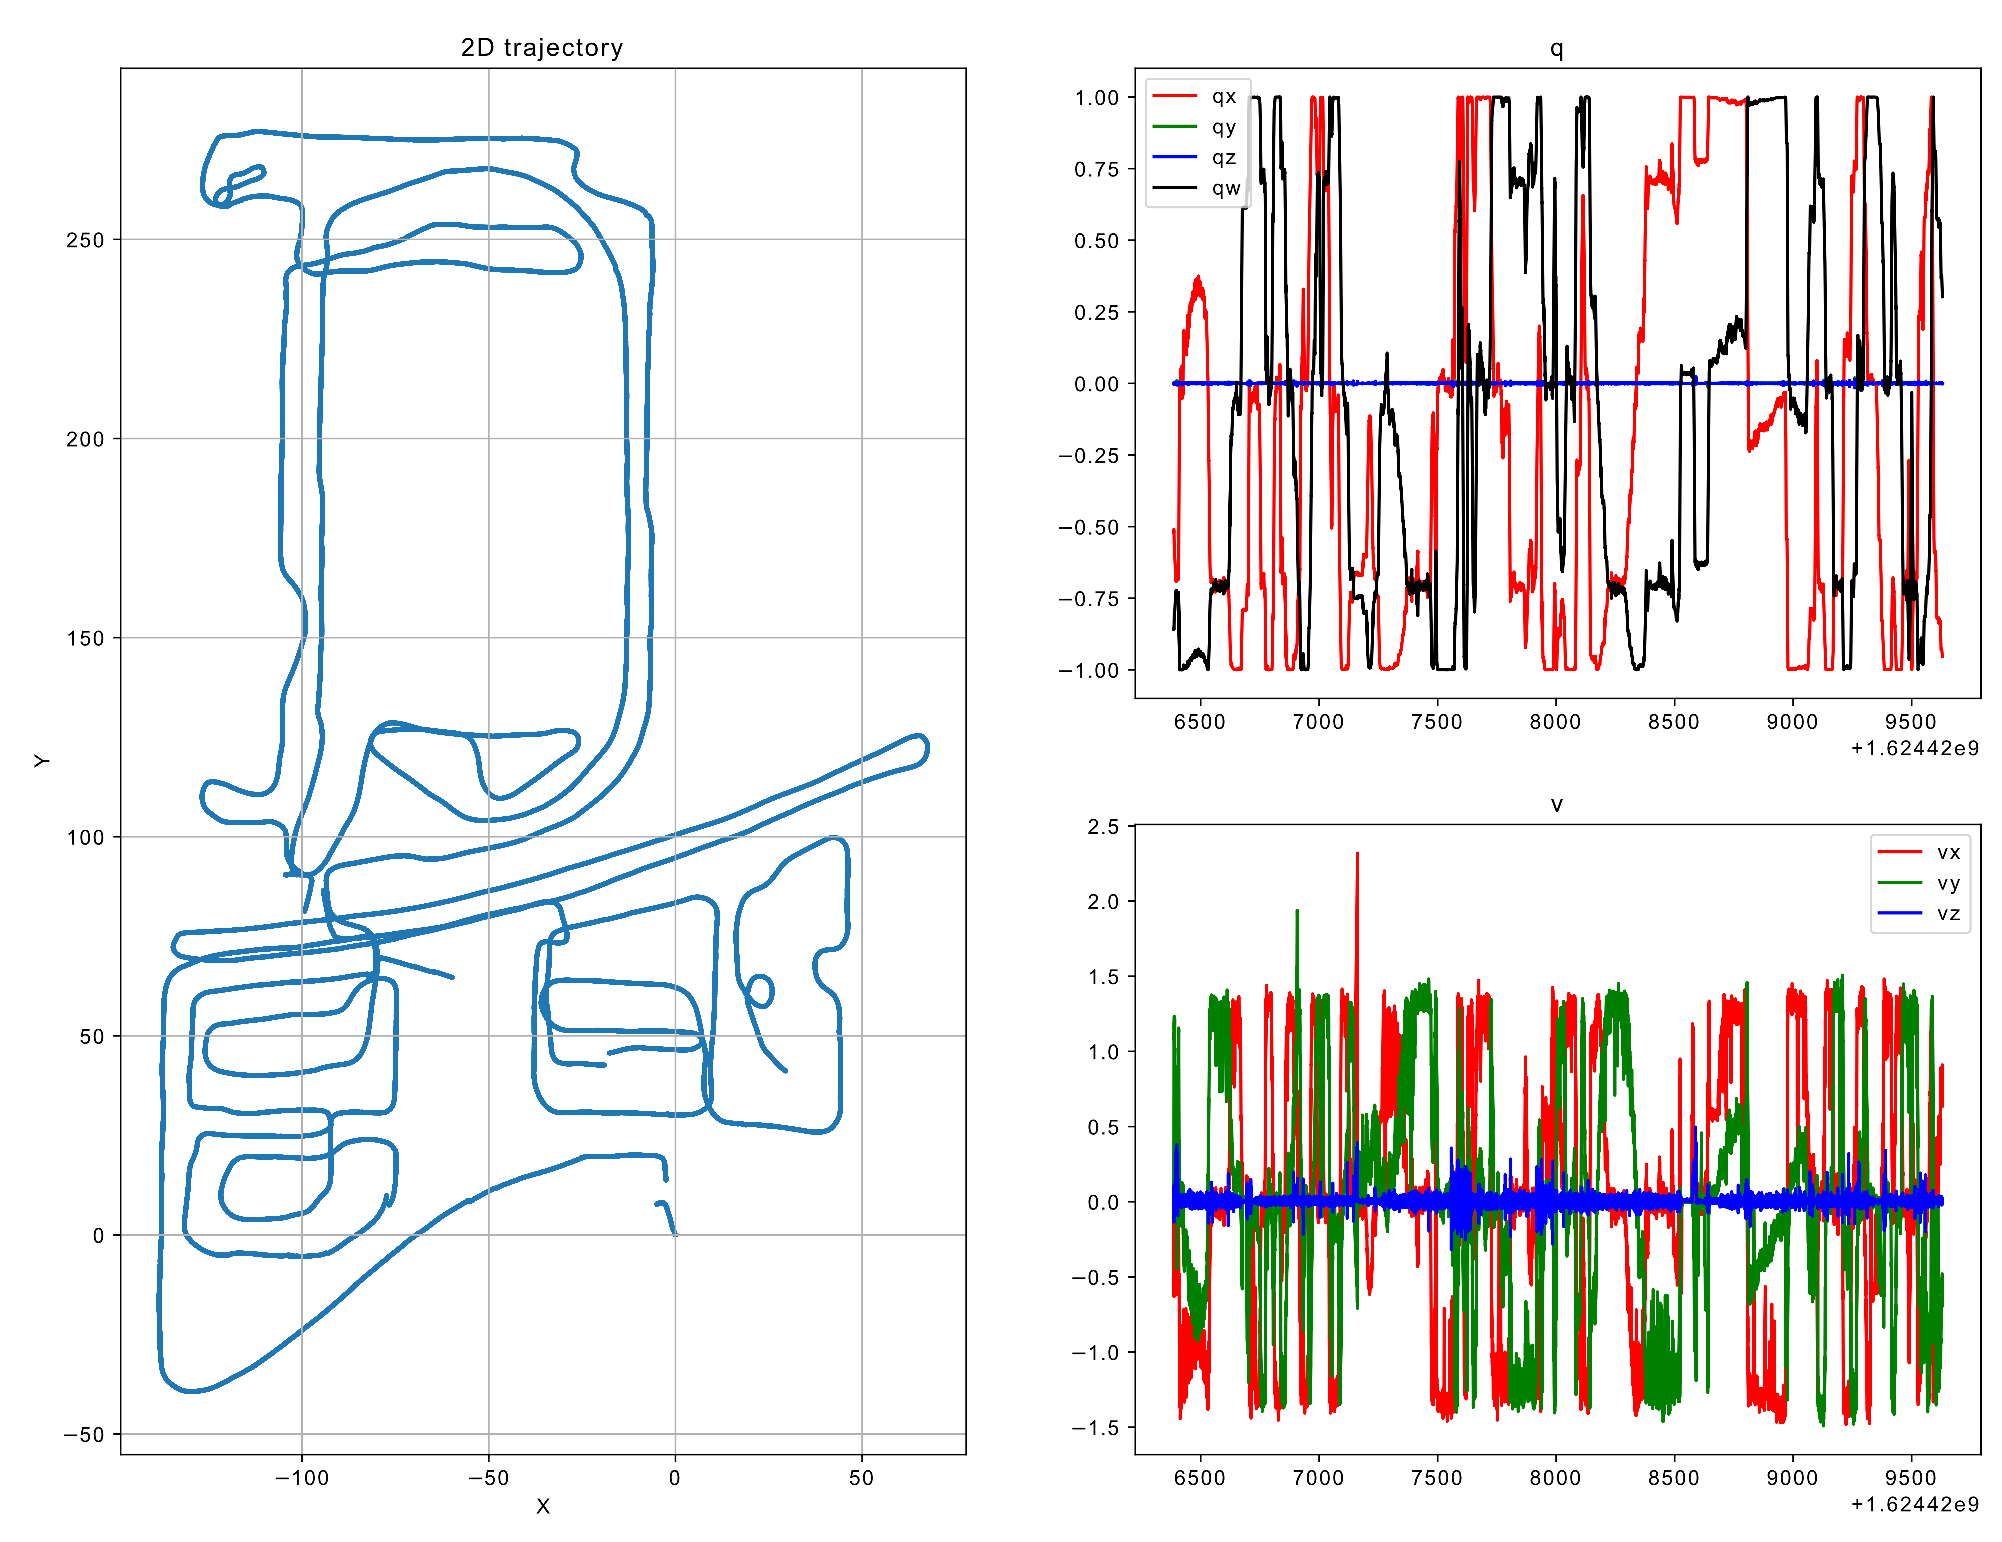
\includegraphics[width=0.8\textwidth]{resources/preintegration/preintegration-gins-out.pdf}
	\caption{GINS results based on pre-integration graph optimization}
	\label{fig:preintegration-gins}
\end{figure}

\section{Summary}
Finally, let's summarize the content of this chapter.

This chapter introduced the fundamental principles of IMU preintegration, including its measurement model, noise model, Jacobian derivation, and handling of biases. Readers can flexibly apply preintegration in practice:

\begin{itemize}
	\item If optimization is not considered, preintegration is completely equivalent to direct integration; it can be used to predict future states.
	\item When used in optimization, preintegration conveniently models the relative motion between two frames. If the IMU bias is fixed, the preintegration model can be greatly simplified. If bias is considered, the preintegrated measurements must be updated accordingly.
	\item The preintegration model can be easily fused with other graph-based optimization models and optimized within the same problem. It also allows flexible configuration of integration time, number of optimized frames, etc., offering more freedom compared to filter-based approaches.
\end{itemize}

Readers are encouraged to compare the content of this chapter with the previous one to understand how two different methods address the same problem. This should be insightful for researchers from various fields.

\section*{Exercises}
\begin{enumerate}
	\item Use numerical differentiation tools to verify the correctness of the Jacobian matrices in preintegration.
	\item Based on the g2o version, implement a Ceres-based version of preintegration DR.
	\item Derive a simplified version of the preintegration model assuming no bias drift. How does it compare to the ESKF approach?
	\item According to the alternative definition in Section~\ref{subsec:4.1.5}, define the preintegration residual, derive its form and Jacobians with respect to each state variable, and discuss whether it offers computational advantages.
	\item Simplify the computation of some Jacobians in preintegration by caching intermediate results to avoid redundant calculations.
	\item In a GINS system based on preintegration, consider how to prevent divergence in position estimates due to prolonged absence of RTK observations. Implement a method to trigger optimization using odometry.
\end{enumerate}

